\documentclass[a4paper]{scrreprt}


%%% PACKAGES %%%

% add unicode support and use german as language
\usepackage[utf8]{inputenc}
\usepackage[ngerman]{babel}

% Use Helvetica as font
\usepackage[scaled]{helvet}
\renewcommand\familydefault{\sfdefault}
\usepackage[T1]{fontenc}

% Better tables
\usepackage{tabularx}

% Better enumerisation env
\usepackage{enumitem}

% Use graphics
\usepackage{graphicx}

% Have subfigures and captions
\usepackage{subcaption}

% Be able to include PDFs in the file
\usepackage{pdfpages}

% Have custom abstract heading
\usepackage{abstract}

% Need a list of equation
\usepackage{tocloft}
\usepackage{ragged2e}

% Better equation environment
\usepackage{amsmath}

% Symbols for most SI units
\usepackage{siunitx}

\usepackage{csquotes}

% Clickable Links to Websites and chapters
\usepackage{hyperref}

% Symbols like checkmark
\usepackage{amssymb}

% Bibliography & citing
\usepackage[
	backend=biber,
	style=apa,
	bibstyle=apa,
	citestyle=apa,
	sortlocale=de_DE
	]{biblatex}
\addbibresource{Referenzen.bib}
\DeclareLanguageMapping{ngerman}{ngerman-apa}

%%% COMMAND REBINDINGS %%%
\newcommand{\tabitem}{~~\llap{\textbullet}~~}

% Define list of equations - Thanks to Charles Clayton: https://tex.stackexchange.com/a/354096
\newcommand{\listequationsname}{\huge{Formelverzeichnis}}
\newlistof{myequations}{equ}{\listequationsname}
\newcommand{\myequations}[1]{
	\addcontentsline{equ}{myequations}{\protect\numberline{\theequation}#1}
}
\setlength{\cftmyequationsnumwidth}{2.3em}
\setlength{\cftmyequationsindent}{1.5em}

% Usage {equation}{caption}{label}
\newcommand{\indexequation}[3]{
	\begin{align} \label{#3} \ensuremath{\boxed{#1}} \end{align}
	\myequations{#3} \centering \small \textit{#2} \normalsize \justify }

%%% PATH DEFINITIONS %%%
% Define the path were images are found
\graphicspath{{./img/}{./pdf/}}

%%% TITLEPAGE %%%

\title{Projektdokumentation}
\subtitle{PAWI HS18}
\author{Pascal Baumann, Dane Wicki}
\publishers{Richard Wetzel}
\date{\today}

%%% DOCUMENT %%%

\begin{document}
\pagenumbering{Roman}
\begin{titlepage}
\maketitle
\end{titlepage}

\renewcommand{\abstractname}{Management Summary}
\begin{abstract}
	Hier könnte ihr Management Summary stehen.
\end{abstract}

\section*{Versionskontrolle}

\begin{tabularx}{\textwidth}{|c|c|c|X|}
	\hline
	\textbf{Versionsnummer} & \textbf{Kürzel} & \textbf{Datum} & \textbf{Beschreibung} \\
	\hline
	0.1 & PB & 10.09.18 & Erste Versionierung \\
	\hline
	0.2 & PB & 16.11.18 & Zwischenabgabe an Betreuer \\
	\hline
	0.3 & PB & 23.11.18 & Ende Sprint 5\\
	\hline
\end{tabularx}

\tableofcontents

\clearpage
\pagenumbering{arabic}
\chapter{Einleitung}
% TODO Einführungstext

\section{Aufgabenstellung und Zielsetzung}
Ziel dieser Arbeit ist es zu Untersuchen, \textquotedblleft inwiefern ein Gebäude mittels Augmented Reality vor Ort selbst dargestellt werden kann, um interessierten Nutzern ein besseres Verständnis des Neubaus zu vermitteln.\textquotedblright Es muss untersucht werden, welche Technologien geeignet für den Ausseneinsatz zur Verfügung stehen. Es soll darauf geachtet werden, dass die Applikation einen Nutzten für die breitere Gesellschaft aufweist. Denn im Moment werden in der Schweiz bei ordentlichen Bauvorhaben noch Bauprofile aufgestellt, welche einen Überblick über die Dimension des Gebäudes wiedergibt, so soll in Zukunft eine Applikation im Sinne dieser Arbeit diese Konstrukte erweitern.
\bigbreak
Es ist zu Beginn der Arbeit noch unklar, welche Geräte für einen Ausseneinsatz verwendet werden können. Daher muss eruiert werden, welche Einsatzgeräte für diese Zwecke brauchbar sind. Weiter soll für die jeweilige Plattform ein geeignetes AR Framework gefunden oder erstellt werden, und schlussendlich die prototypische Applikation selbst entwickelt werden.
\bigbreak
Die vorliegende Arbeit beschäftigt sich stark mit der Fragestellung, inwiefern eine solche Applikation mit heutigen Geräten umsetzten lässt. Zudem sollen dabei deren Schwächen, sowie Vorteile aufgezeigt werden.
\chapter{Grundlagen}
\label{ch:StandDerForschung}

% TODO some Text about what we will do in this chapter...

\section{Technologische Grundlagen}

\subsection{Historische Entwicklung}

Als Augmented Reality (dt. erweiterte Realität) versteht man das Vermitteln von Zusatzinformationen über die Umgebung in Form von Animationen, Einblendungen und Tonwiedergaben. In den meisten Fällen wird dies über Smartphones oder Computer bewerkstelligt, es existieren jedoch auch spezialisierte Geräte wie die Microsoft HoloLens oder Google Glass.

% TODO Science Ficiton, Head-Mounted Displays, Azuma

Der Term wurde erstmals von \citeauthor{Milgram1994} im Jahre 1994 detailliert definiert, wobei sie die Vermischung der realen und virtuellen Welt betrachten und wohin die Technologie Augmented Reality fällt (siehe \ref{fig:RVContiinum}):

\vspace{1em}

\textquotedblleft the above-mentioned broad definition of Augmented Reality –  \textquoteleft augmenting natural feedback to the operator with simulated cues\textquoteright\ – is quite clear. Also noteworthy in this figure is the corresponding concept of Augmented Virtuality (AV), which results automatically, both conceptually and lexically, from the figure. \textquotedblright\ \parencite{Milgram1994}

\begin{figure}[htb]
	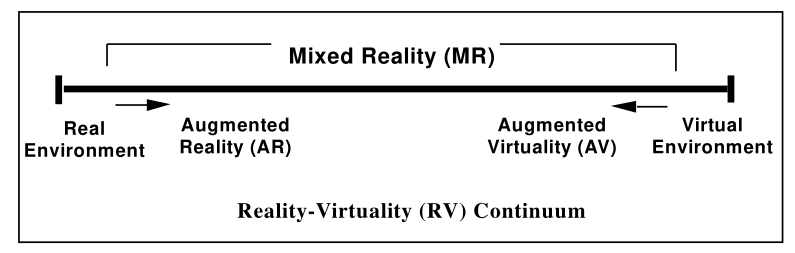
\includegraphics[keepaspectratio, width=\textwidth]{MR_milgram.png}
	\caption{Simplified representation of a RV continuum \parencite{Milgram1994}}
	\label{fig:RVContiinum}
\end{figure}

Fünf Jahre nach Milgram veröffentlichten \citeauthor{Kato1999} ihre Ergebnisse zu einem Marker-basierten AR Konferenzsystem. Sie lösten dabei das Problem der Registrierung (wo befindet sich der Benutzer, oder besser gesagt dessen Augen), und das Ermitteln der Pose (wie ist die Orientierung der virtuellen Kamera in Bezug zur Umwelt) über Marker mit einer fixen Grösse \parencite{Kato1999}. Das System war stationär mit Computern realisiert. In den folgenden Jahren wurden Versuche mit  mobilen Prototypen durchgeführt, dies blieben jedoch in der Grösse von Rucksäcken, und gebrauchten Notebooks mit der entsprechenden Rechenleistung (siehe Abbildung \ref{fig:MobileSysteme}).

\begin{figure}[h!]
	\centering
	\begin{subfigure}[t]{0.45\textwidth}
		\centering
		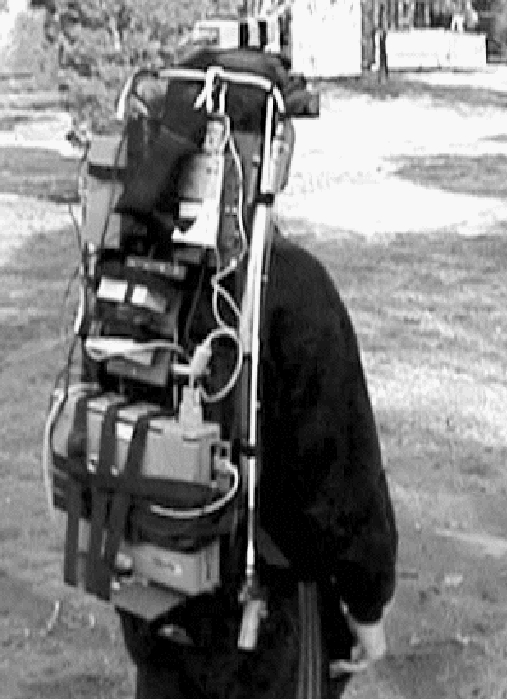
\includegraphics[keepaspectratio, width=0.4\textwidth]{tinmith2.png}
		\caption{Das TINMITH2 System \parencite{Thomas1999}}
	\end{subfigure}
	\quad
	\begin{subfigure}[t]{0.45\textwidth}
		\centering
		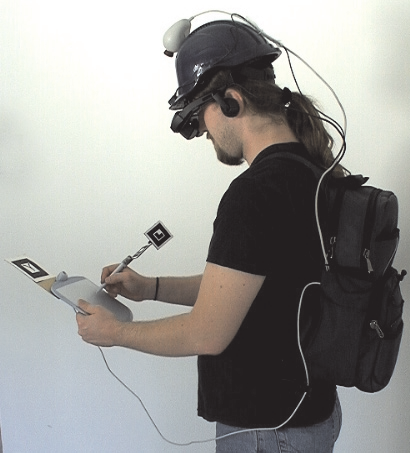
\includegraphics[keepaspectratio]{Studierstube2001.png}
		\caption{Interaktion mit der StudierStube Applikation \parencite{Reitmayr2001}}
	\end{subfigure}

	\begin{subfigure}[b]{0.45\textwidth}
		\centering
		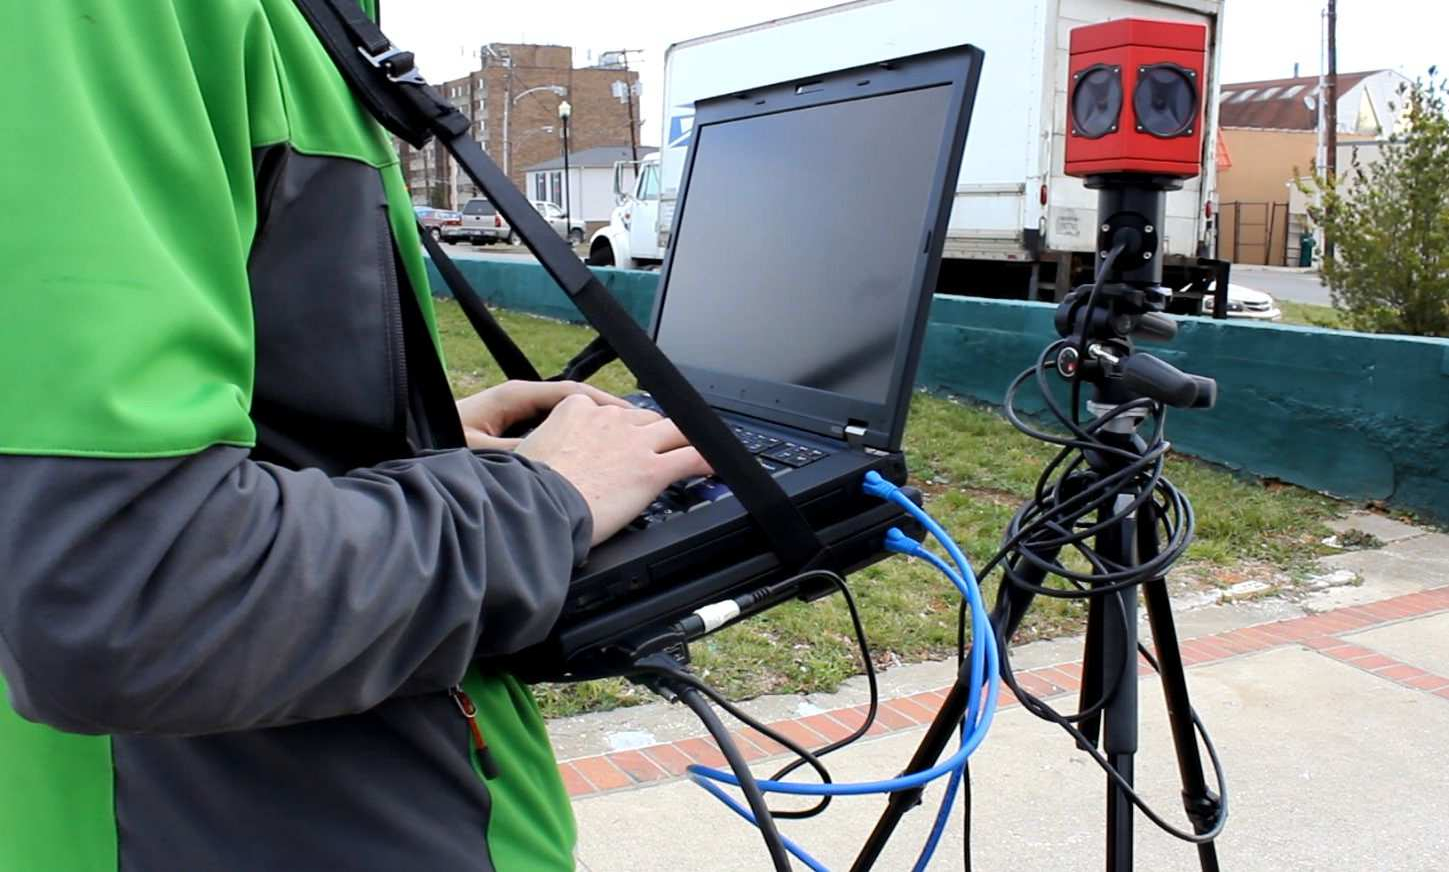
\includegraphics[keepaspectratio, width=0.6\textwidth]{LiveMobilePanoramicAR.png}
		\caption{\parencite{Cote2013}}
	\end{subfigure}
	\quad
	\begin{subfigure}[b]{0.45\textwidth}
		\centering
		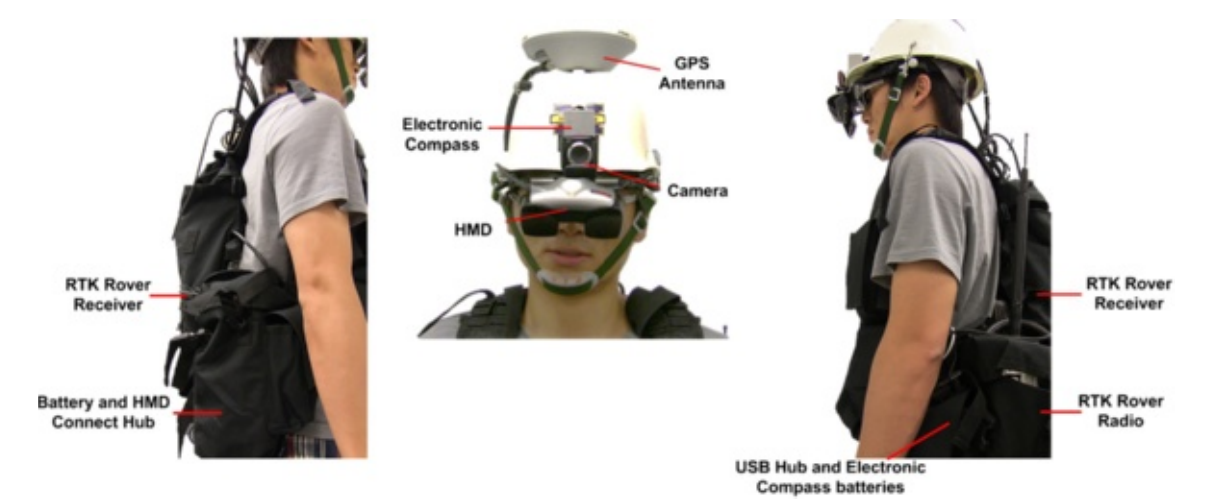
\includegraphics[keepaspectratio, width=0.8\textwidth]{ARMOR_System2013.png}
		\caption{Das ARMOR System \parencite{Dong2013}}
	\end{subfigure}
	\caption{Beispiele verschiedener mobiler Systeme}
	\label{fig:MobileSysteme}
\end{figure}

Ein grosser Durchbruch wurde deshalb von \citeauthor{Klein2009} erbracht, welche einen PTAM (Parallel Tracking and Mapping) Algorithmus auf einem iPhone 3G implementierten. Dieser war in der Lage sowohl in Räumen wie ausserhalb von Gebäuden, nach einer Initialisierungsphase die Lokalisierung von einem Marker loszulösen und die Pose der Kamera über \textquotedblleft Key Features\textquotedblright\ zu ermitteln \parencite{Klein2009}. Seither wurde auf diesem Gebiet weiter entwickelt und Algorithmen dieser Art sind unter dem Namen SLAM (Simultaneous Location and Mapping) zusammengefasst, dazu existieren verschiedene Frameworks welche diese nativ mitbringen (Kudan, wikitude).

\subsection{Konzepte}

\subsubsection{Markerbasierte Initialisierung}
Ein wichtiges Problem, das jede AR Applikation lösen muss, ist die Registration. Damit ist gemeint, dass die Applikation Koordinatensysteme und Ausrichtung der virtuellen Welt mit der realen Welt abgleichen und überwachen muss.

Optische (d.h. Analyse der Kameradaten) Methoden werden von den gängigen Frameworks von Grund auf unterstützt. Zu diesen optischen Methoden gehören auch Marker. Ein Marker ist in den besten Fällen ein selbst unter Rotation und Scherung verformtes, eindeutig identifizierbares Muster, kann aber im Prinzip jegliches Bild sein. Ein guter Marker hat vorzugsweise einen hohen Kontrast im Grauspektrum, und grosse, komplexe Elemente ohne feine Details (welche auf Distanz verschwimmen oder verloren gehen) \parencite{Kudan2016}.

Die eigentliche Erkennung der Marker geschieht mit Algorithmen der Computer Vision (Kantenerkennung, Eckerkennung), worauf ein erkannter Marker mit einer Datenbank von bekannten abgeglichen wird. Danach kann über jenen einzelnen Marker sowohl Positionierung wie auch Lokalisation geschehen.

\subsubsection{Markerless}
Da beim Markerbasierten Tracking die namensgebenden \textquotedblleft Fiducial Markers\textquotedblright\ immer im Fokus der Kamera bleiben müssen, möchte man, falls möglich, diese gar nicht erst einsetzen müssen. Dies kann auf zwei verschiedene Arten erreicht werden: Modell-basiert und Feature-basiert \parencite{Ziegler2009}.

Ein modellbasiertes Tracking generiert aus einem physischen Objekt ein dreidimensionales, digitales Modell, dieses wird danach verwendet, um die Pose zu kalkulieren. Üblicherweise werden diese Modelle aufgrund der Kanten oder Ecken des Objektes berechnet, Kanten sind dabei vorzuziehen, da Sie gegenüber wechselnden Lichtverhältnissen robust sind und durch den Computer effizient gefunden werden können \parencite{Zhou2008}. Dies bedeutet jedoch nicht, dass dies die einzigen beiden Möglichkeiten für ein Modellbasiertes Tracking sind, sowohl \citeauthor{PauloLima2017} wie auch \citeauthor{Cote2013} gebrauchen in ihren Arbeiten Systeme, welche von Punktewolken ausgehend die jeweilige Pose ausrechnen.

Die Feature-basierte Methode extrahiert interessante Punkte eines Bildes und versucht diese auf subsequenten Bildern wiederzufinden. Wie diese Punkte identifiziert werden hängt von der gewählten Methode ab. Bei SIFT (scale-invariant feature transform) sind dies beispielsweise die Minima/Maxima mehrerer Gaussschen Weichzeichnungsfunktionen \parencite{Lowe1999}. Bei nachfolgenden Bildern werden wieder Features bestimmt und mit den vorhergegangen abgeglichen. Erschwert wird der Prozess dadurch, dass zwei Bilder nicht unbedingt durch Transformationen (Rotation, Skalierung, Scherungen) ineinander überführt werden können. Es müssen also Features gefunden und erkannt werden, welche gegen solche Transformationen resistent sind.

\subsubsection{SLAM}
Wie im vorherigen Paragraf erklärt, wird zwischen zwei Markerless Tracking Methoden unterscheiden. Eine spezifische, die sogenannte SLAM Methode, wird in diesem Paragraoh näher erklärt. Diese Methode identifiziert, mit Computer Vision, Feature-Points (ein Bildpunkt der sich durch seine lokale detaillierte Umgebung von anderen Punkten desselben Bilds hervorhebt), sowie deren Abhängigkeiten zueinander (Location) und fasst diese in einer Karte zusammen (Mapping). Sollte nun die Pose verloren gehen (durch einen Unterbruch des Kamerastream oder zu schnelle Bewegungen), muss nur ein Teil der vorherigen Karte wiedergefunden werden, um die Position wieder zu bestimmen. Dieser Ansatz wird \textquotedblleft Simultaneous Location and Mapping\textquotedblright (dt. Simultanes Erkennen und Kartografieren) genannt.

\subsubsection{GPS}
% TODO Write about GPS System

\section{Anwendungen}

Der Einsatz von virtueller oder gemischter Realität ist für die Fachbereiche Medizin und Konstruktion sehr interessant. Wie \citeauthor{Piroozfar2018} beschreiben, bringt ein solcher Einsatz in der Konstruktionsindustrie verbesserte Kommunikation, besseres Verständnis eines Projektes, präzisere Planung, schnellere Entscheidungsfindung, und alles in allem eine erhöhte Sicherheit und Effizienz \parencite{Piroozfar2018}. \citeauthor{Pelargos2017} sehen den Mehrwert für die Medizin in Planung einer Operation und verbesserte, da nicht gleich kritisch, Ausbildung der beteiligten Fachkräfte \parencite{Pelargos2017}. Im Vergleich zu traditionellen pädagogischen Methoden, bietet MR ein Potential den Lernenden greifbarer zu motivieren, und gleichzeitig dessen räumliches Vorstellungsvermögen und technische Fähigkeiten zu verbessern. Weiter erwarten Sie eine erhöhte Retention des gelernten, da der Kontext des Lernstoffs direkter bei der Anwendung dessen ist.

Beide Gruppen identifizieren jedoch dasselbe Problem für die geringe Adoption von AR in deren relevanten Felder: ein Existieren von performanter, komfortabler Hardware, welche einen bezahlbaren Preis besitzt und für diese Felder geeignet sind in Bezug auf Komfort und anderen Anforderungen. Im Moment sind solche Geräte ein Nischenprodukt, was dazu führt, das Entwicklung für ein solches Produkt ein erhebliches Risiko darstellt (\cite{Piroozfar2018}, \cite{Pelargos2017}).

Im Bereich der Unterhaltungsindustrie hat AR hingegen schon längst Einzug gehalten. Zwei der grössten Spiele (Ingress und Pokémon Go!) wurden von Niantic Labs entwickelt und besitzen Nutzerzahlen in Millionenhöhe, beide spielen in einer Spielwelt die entweder auf unserer basiert (Pokémon Go!) oder spielen in einem Paralleluniversum (Ingress) in welchem Aktionen in der realen Welt Auswirkungen besitzt. Dennoch plagen beide das gleiche Problem: Betrug der Geolokation der spielenden Geräte und ein fehlendes Endziel (\cite{MRRX2015} und \cite{KamelBoulos2017}). Dies führte zu einer Stagnation und Verlust von Spielern, nachdem der Initiale Ansturm vorüber war (\cite{Arif2017}, \cite{KamelBoulos2017}), dennoch trugen diese Spiele Massgeblich dazu bei ein öffentliches Verständnis von AR zu bilden. Es darf daher davon ausgegangen werden, das dadurch die Hürde für die Entwicklung neuer Spiele tiefer geworden ist.

\subsection{Building Information Modelling}

Auch im Bereich des BIM (Building Information Modelling) wurde im Zuge der Fortschritte in AR verschieden Lösungen erarbeitet. Spezialisierten Fachlösungen wie beispielsweise die DAQRI Smart Glasses (welche für AR und BIM im Industrieumfeld eingesetzt werden) \parencite{DAQRI2018}, welche das Format Autodesk BIM 360 direkt im Gebäude darzustellen um Sanitär-, Ventilation- und Elektroleitungen auf dem Gelände direkt darzustellen und Planungsprobleme zu identifizieren. Diese befindet sich im Moment jedoch noch im \textquotedblleft Early Adopter\textquotedblright-Status, und ist dementsprechend nicht ausgereift.

Das Team von Auto AR \parencite{Opperman2015} entwickelten ein System, welches es einem Benutzer erlaubt Neu- und geplante Bauten aus einem Auto zu begutachten. Dazu montierten sie auf einem Personenwagen eine omnidirektionale Panoramakamera, welche ihre Daten an einen im Wagen befindenden Laptop überträgt. Dieser bereitet das Bild auf, platziert das zu betrachtende Gebäude in der virtuellen Welt, und speist diese virtuelle Welt an ein Oculus Rift, welche vom Probanden getragen wird. Damit sieht dieser sowohl eine Projektion der reelen Welt, wie auch das geplante Gebäude an dessen Stelle.

Eine andere Richtung wurde vom Frauenhofer Institut in Darmstadt \parencite{Olbrich2013} eingeschlagen. Sie entwickelten ein BIM Framework welches erlaubt, über bestehende Gebäudebestandteile Mehrinformationen anzuzeigen, und dies sowohl auf stationären Kioskcomputern, wie auch auf mobilen Geräten, welche sich im Gebäude bewegen. Sie entwickelten dafür eine Server Client Infrastruktur, welche die Berechnungen der Pose und Szenendarstellung auf den Server auslagert, und so die schwächeren Endgeräte entlastet. Ihre dafür eigens entwickelte Infrastruktur erlaubt den Benutzer ebenfalls, Notizen über ein Objekt dynamisch auf diesem zu platzieren, sodass dies auf allen anderen Endgeräten ebenfalls erscheint.

\section{Benutzerführung in AR Applikationen}
In der heutigen Zeit ist die User Experience (dt. Erfahrung der Interaktion des Benutzers mit einem System) ein zentraler Bestandteil in der Entwicklung von Applikationen. Es gibt kaum noch erfolgreiche Anwendungen, welche nicht ein spezielles Team für die Entwicklung der User Experience besitzen.

Für die Entwicklung einer zweidimensionalen Applikation gibt es bereits heute genaue Vorgaben und Vorgehensmodelle, wie eine solche Applikation eine gute User Experience erreichen kann. Leider können nicht alle Vorgaben und Vorgehensmodelle auch für eine dreidimensionale Applikation verwendet werden. Da unserer Applikation eine Augmented Realitiy Applikation wird, trifft dies speziell zu.
Für die Entwicklung einer guten User Experience für eine AR Applikation gibt es jedoch verschiedene Ansätze und Empfehlungen, welche von verschiedenen Unternehmen veröffentlicht wurden. 

\subsection{User Centered Design}
\begin{figure}[h!]
	\centering
	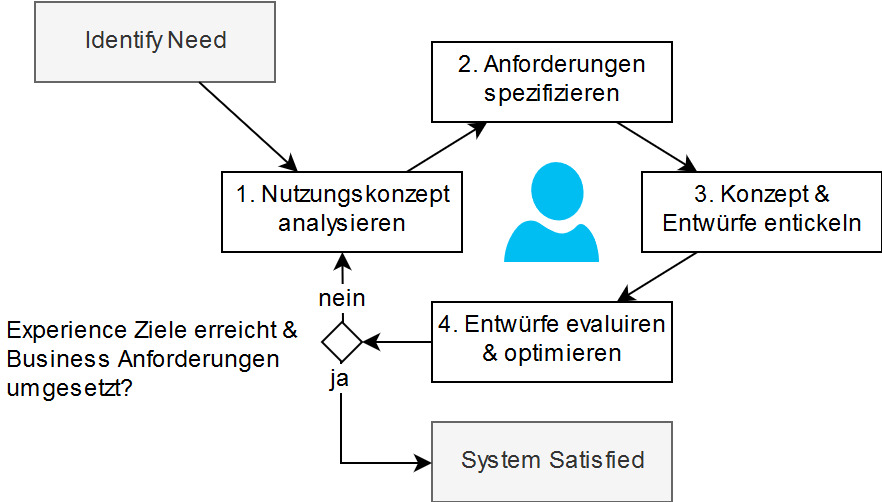
\includegraphics[keepaspectratio,width=0.8\textwidth]{UserCenteredDesign}
	\caption{Phasenmodell des ISO Standart 9241-210:2010 \parencite{ISO9241}}
\end{figure}

Um eine möglichst optimale User Experience zu erreichen, kann nach den Methodiken des Standards ISO 9241-210:2010 (fortan als User Centered Design bezeichnet) vorgegangen werden. Dies ist ein iteratives Vorgehen, bei dem die Benutzer im Zentrum stehen. Dies mit ihren Zielen, Bedürfnissen und Erwartungen über den gesamten Entwicklungsprozess hinweg. 
Jede Iteration dieses Prozesses durchläuft vier Phasen, bevor das Produkt in eine finale Version kommt.

Diese Methodik für die Ermittlung einer guten User Experience kann auch bei der Entwicklung einer AR Applikation verwendet werden.
In Phase 3 werden im User Centered Design zu Beginn meist Prototypen auf Papier entwickelt, mit welchem sich der Benutzter konzeptuell durch die Applikation navigieren muss. Diese Papierprototypen sind für eine dreidimensionale Applikation schwieriger zu gestalten und erschweren dadurch den Prozess. Bedingt durch diese Komplikation, ist der ganze Ablauf des User Centered Design teurer und komplexer (\cite{ISO9241}).

\subsection{Graphical User Interface Konzepte}
Im Rahmen des User Centered Designs gibt es zudem Richtlinien und Verhaltensweisen der graphischen Benutzeroberfläche.
Auch hier gilt, was bei zweidimensionalen GUI's funktioniert, muss nicht oder kann nicht zwingend bei einer AR Applikation verwendet werden. Um dem Benutzer die Interaktion mit der AR Applikation möglichst einfach und intuitiv zu gestalten, müssen folgende Punkte mit Sicherheit beachtet werden.

\subsubsection{Bildschirmflächenoptimierung}
Eine AR Applikation vermittelt den Eindruck, als ob die physikalische Welt die Limitierung der Applikation sei, in Wahrheit ist jedoch der Bildschirm des Anzeigegerätes die eigentliche Limitierung .
Der Benutzer möchte also möglichst wenig von seiner eigentlichen Intention, zum Beispiel der Besichtigung eines Gebäudes von aussen, abgelenkt werden. Dies setzt voraus, dass die Informationen sowie Interaktionsmöglichkeiten weitgehendst konsolidiert werden.

\subsubsection{Vereinfachter Einstieg}
Selbst in einer zweidimensionalen Applikation ist die Einarbeitung in eine Applikation teilweise sehr schwierig und zeitaufwendig. In einer dreidimensionalen Applikation gestaltet sich dies jedoch noch um einiges schwieriger und ist meist mit einer grösseren Lernkurve verbunden, weshalb der Einstieg ein noch wichtigerer Aspekt bei der Entwicklung sein muss.

\subsubsection{Vorhersehbarkeit}
Ein Benutzer bringt durch seine Bildung wie auch seine Herkunft schon Erwartungen mit. Diese antrainierte Verhalten sollte eine Applikation wo immer möglich nutzen und sinnvoll wiederverwenden. Als antrainiertes Verhalten gelten zum Beispiel Gesten zur Vergrösserung und Rotation einer Anzeige. Wo immer möglich sind solche intuitiven Verhalten einer Interaktion durch Buttons und Menüs vorzuziehen,

\subsubsection{Hinweise}
Der Mensch sucht stets nach Hinweisen und Signalen. Dieses Verhalten widerspiegelt sich auch in alltäglichen Situationen wie beispielsweise einer Bahnfahrt, auf welcher wir stets nach Symbolen und Hinweise für die Nächste Haltestelle oder Ausfahrt Ausschau halten.
Solche Hinweise sollen in einer AR Applikation den Benutzer ermutigen die Applikation noch weiter zu erkunden.
Diese Hinweise müssen nicht zwingend Texte sein, so kann auch ein Pfeil in die Richtung deuten, in welche sich das anzuzeigende Objekt befindet, sobald dieses aus dem Bildschirm tritt.

\subsubsection{Vielfältige Benutzer}
Eine AR Applikation soll stets für eine Vielzahl von Benutzer brauchbar sein. Dies soll besonders berücksichtigt werden. Es soll dabei Acht auf Behinderungen wie Farbenblindheit oder ähnliche Konditionen gegeben werden (\cite{AppleGuideline2018}, \cite{GoogleGuideline2018}, \cite{GoogleIO2018}, \cite{BerfinAyhan2017}).

\chapter{Lösung}
Im folgenden Kapitel wird die Lösung beschrieben. Es soll ein Überblick über die Umsetzung der Applikation bieten. Eine detaillierte Beschreibung ist in Kapitel \ref{sec:SysSpec} zu finden. Es wird zudem ein alternatives Konzept vorgestellt, welches nicht weiter verfolgt wurde.

\section{Konzeptionelle Idee}
Wie in Kapitel \ref{ch:StandDerForschung} beschrieben, kann eine AR Applikation Markerless oder Markerbasiert sein. Dabei gibt es auch bei diesen zwei Kategorien unterschiedliche Möglichkeiten diese zu realisieren. Müssen beim Markerbasierten Tracking für die Initiierung und Platzierung ein Marker verwendet werden, so geschieht dies nicht beim Markerless Tracking. Da Markerless Tracking jedoch nicht aus dem Nichts etwas auf dem Bildschirm darstellen kann, muss beim Markerless eine Alternative zum Marker gefunden werden. Dies kann beispielsweise die Erkennung von Flächen sein \parencite{GoogleARCore2018} oder auch Lokalisierungssensoren.
Um eine AR Applikation zu entwickeln, welches ein Gebäude in der realen Umgebung darstellt, würden sich potenziell beide Lösungen, also auf Marker wie auch Markerless basierend, anbieten.
\bigbreak
Das Konzept einer auf Lokalisierungssensoren basierte Lösung sieht vor, dass das darzustellende Gerät über folgende zusätzliche Komponenten verfügt: 
\begin{enumerate}
	\item Lokalisierungssensor (GPS/GLONASS/BEIDOU/GALILEO Sensor)
	\item Kompass
	\item Gyroskop
\end{enumerate}

Bei dieser Lösung werden die Lokalisierungssensoren sowie der Kompass dazu verwendet die Positionierung des darzustellenden Gebäudes zu berechnen. Die lokalen Bewegungen des Anzeigegerätes würden mithilfe des Gyroskops ausgelesen, und dazu verwendet das Gebäude an Ort und Stelle zu halten.
Nachteil dieser Methode liegt darin, dass die Anzeige nun abhängig von drei Sensorwerten ist, welche selber jeweils eine Ungenauigkeit aufweisen und damit Fehler ins System einbringen. Dieser Umstand kann dazu führen, dass das anzuzeigende Gebäude nicht immer an der exakten Position dargestellt wird.

\section{Applikationsablauf}
Die Applikation durchläuft verschiedene Schritte, damit sie dem Benutzer das Modell in der Umgebung an der korrekten Position anzeigen kann. Diese Schritte sind anhand der Abbildung  \ref{fig:Ablaufdiagramm} grafisch ersichtlich.

\begin{figure}[h!]
	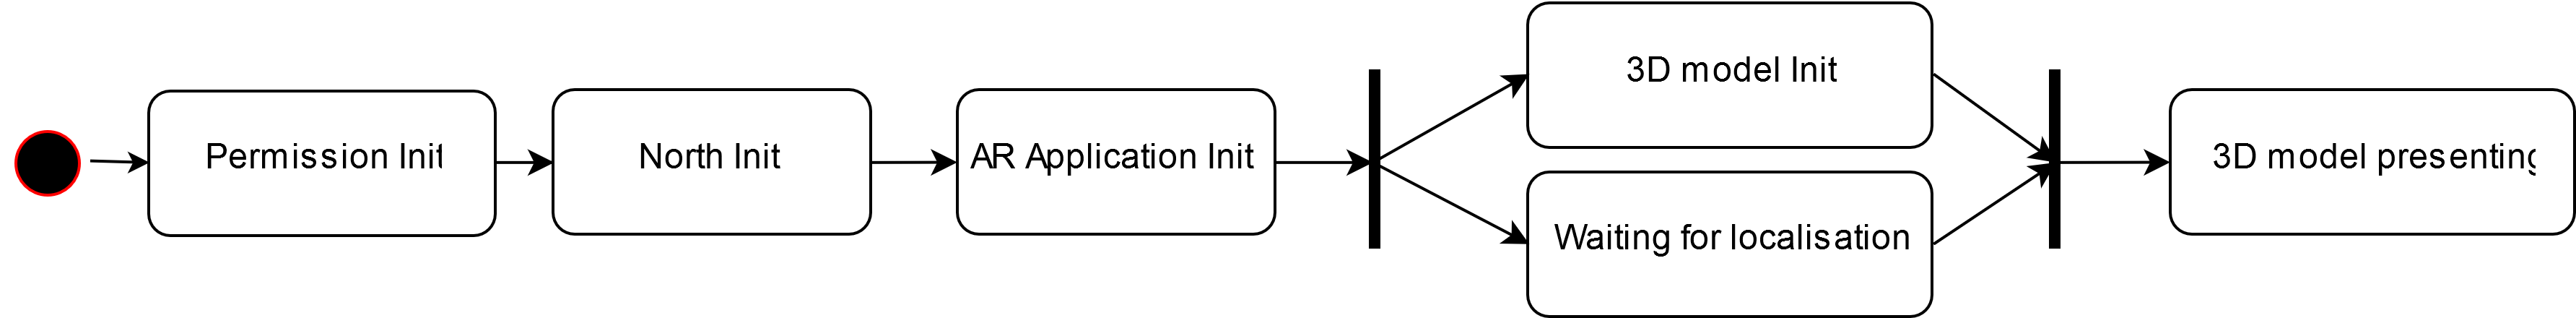
\includegraphics[keepaspectratio, width=\textwidth]{AblaufdiagrammARApplikation.png}
	\caption{Ablaufdiagramm der AR Applikation}
    \label{fig:Ablaufdiagramm}
\end{figure}

\subsection{Permission Init}
Sobald die Applikation startet, werden diverse Berechtigungen überprüft. Sind gewisse Berechtigungen nicht vorhanden, so werden diese in diesem Status beim Benutzer nachgefragt. Hierfür wird dem Benutzer alle fehlenden Berechtigungen in einer Liste dargestellt. Damit der Benutzer nicht in einer Endlosschlaufe die Berechtigungen ablehnt, wird nur einmal nach den Berechtigungen gefragt und anschliessend lediglich auf Wunsch des Benutzers erneut gefragt. Es ist zwingend notwendig, dass der Benutzer diese Berechtigungen zulässt da sonst die ganze Applikation nicht funktionsfähig ist. Hat der Benutzer allen Berechtigungen zugestimmt oder hat die Applikation schon alle Berechtigungen, wechselt der Status auf den im Kapitel \ref{ch:NorthInit} beschriebenen Zustand. Die Abbildung \ref{fig:PermissionInitStatus} stellt das Grafische Benutzeroberfläche der Abfrage dar.
\begin{figure}[h!]
	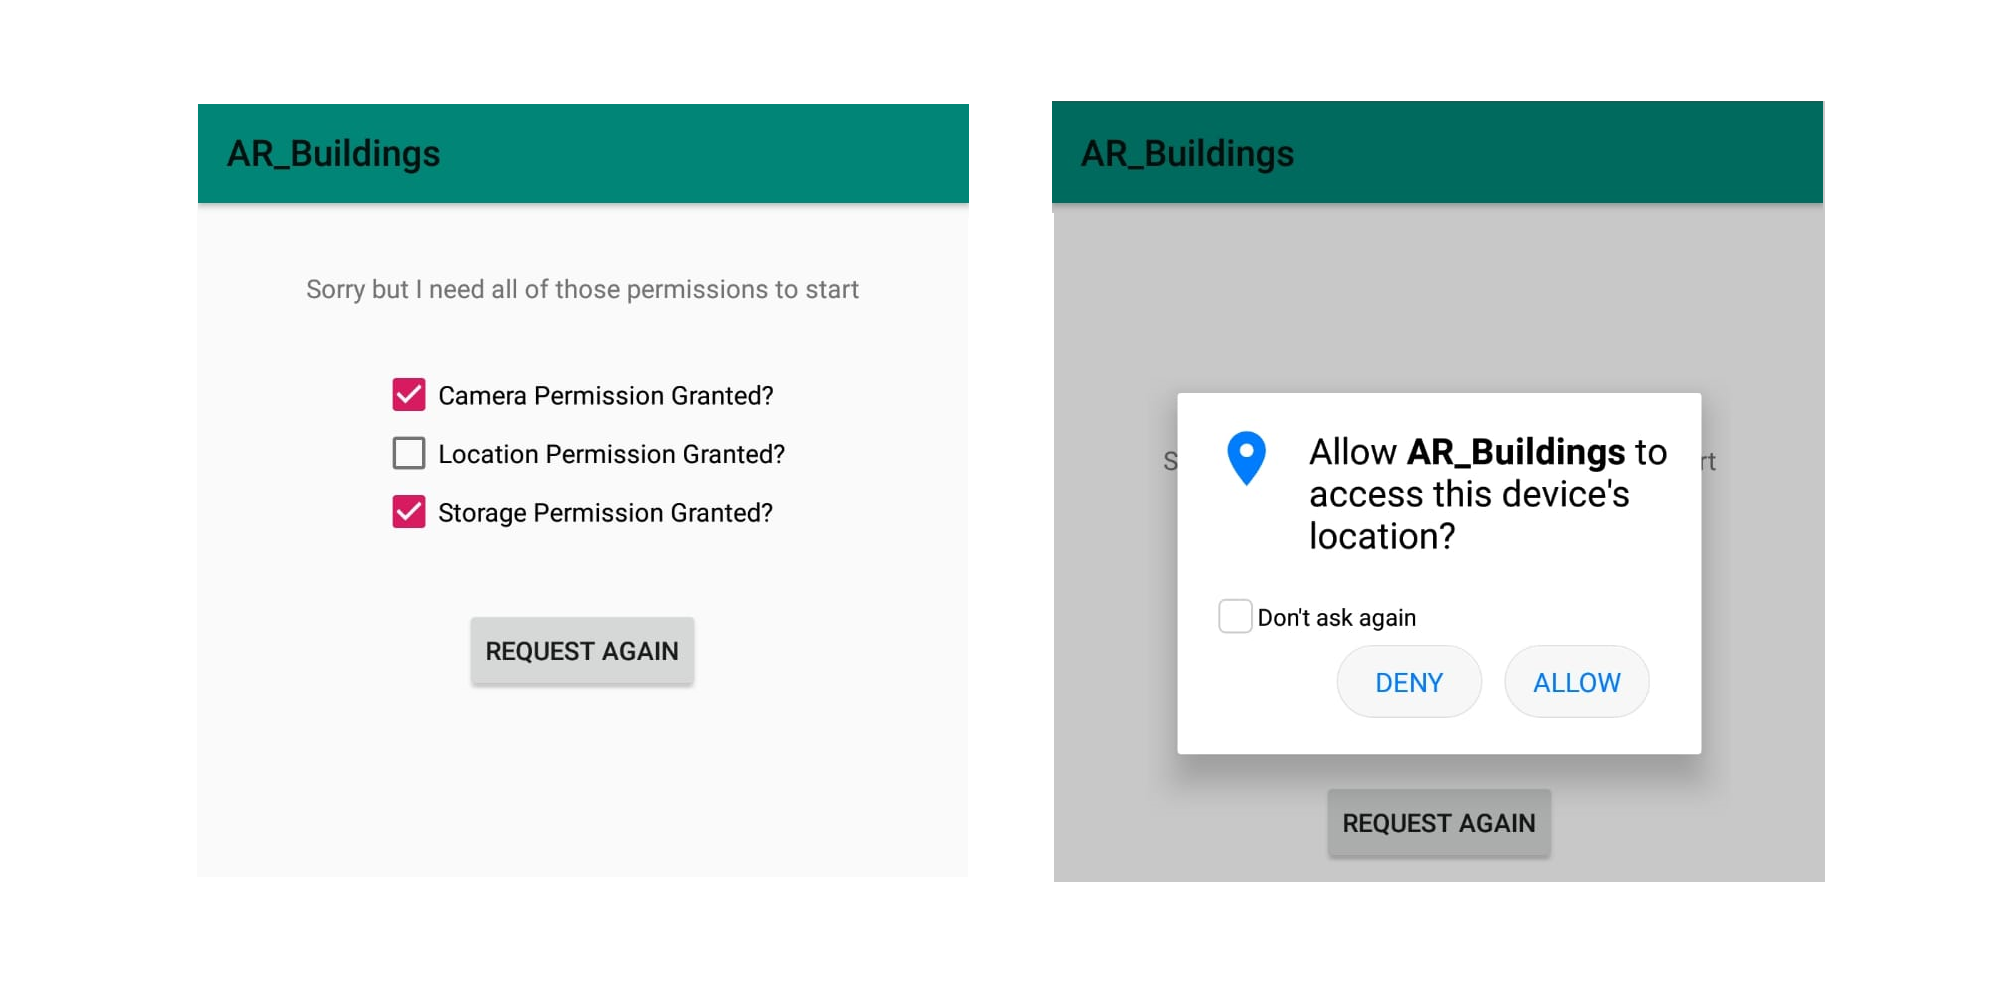
\includegraphics[keepaspectratio, width=\textwidth]{ARBuildingPermissionRequest.png}
	\caption{Darstellung und Abfrage fehlender Berechtigung}
    \label{fig:PermissionInitStatus}
\end{figure}

\subsection{North Init} \label{ch:NorthInit}
In diesem Status wird versucht den Nordpol mittels Kompass herauszulesen. Dabei wird der Benutzer dazu aufgefordert, dass Smartphone nach Norden auszurichten. Dieser Zustand dient dazu, dass nicht ständig der Norden vom Kompasssensor herausgelesen werden muss, was zu einer Steigerung der Genauigkeit führt. Sobald der Benutzer das Gerät genug lange nach Norden ausgerichtet hat, startet die Applikation in den in Kaptiel \ref{ch:ARApplicationInit} beschriebenen Status. In der Abbildung \ref{fig:NorthInitProcess} ist die Grafische Benutzeroberfläche für die Initialisierung dieses Schrittes zu sehen.
\begin{figure}[h!]
	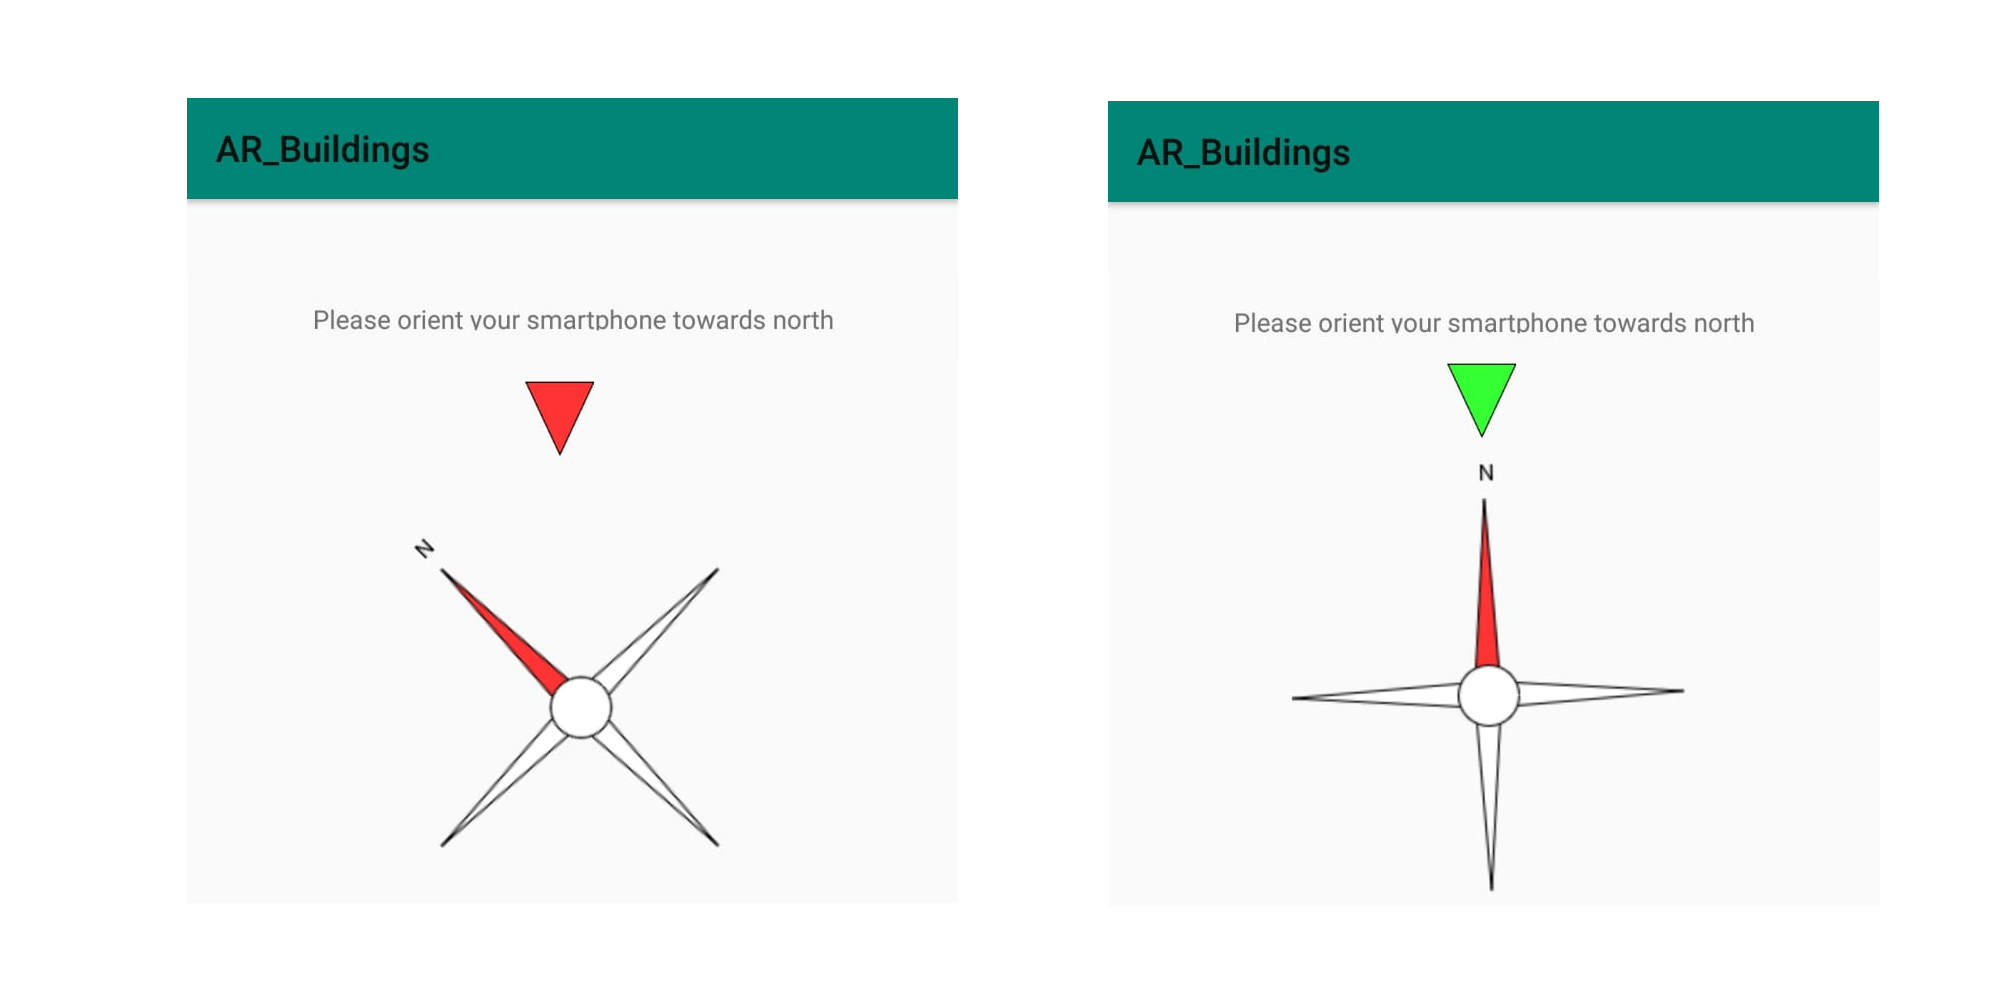
\includegraphics[keepaspectratio, width=\textwidth]{NorthInitProcess.png}
	\caption{Darstellung North Init mit Indikator ob richtige Position erreicht wurde.}
    \label{fig:NorthInitProcess}
\end{figure}

\subsection{AR Application Init} \label{ch:ARApplicationInit}
Kommt die Applikation in diesen Status, werden alle notwendigen Schritte für die Initialisierung der AR Applikation gestartet. Dies bedeutet insbesondere, dass die Kudan AR Welt aufgebaut wird. Zudem abonniert dieser Status den Event, welcher bei Lokalisierungsupdates des Gerätes geworfen wird und wechselt zum Status, welcher in Kapitel \ref{ch:waitingForLocation} beschrieben ist.

\subsection{3D Model Init}
Dieser Status \textquotedblleft 3D Model Init\textquoteright\ erfüllt zum jetzigen Zeitpunkt noch keinen Zweck. Er würde jedoch die Modelle, welche die Applikation darstellen soll von einer Website herunterladen und diese der Applikation bereitstellen.

\subsection{Waiting for localisation} \label{ch:waitingForLocation}
In diesem Schritt wird gewartet, bis eine valide Lokalisierungsposition vom Gerät zurückgegeben wird. Die Position wird als valide betrachtet, sobald sie genügend genau ist. Der Benutzer wird auch hier über den Zustand der Applikation informiert (siehe Abbildung \ref{fig:KoordinationNotFound}), indem eine Grafische Darstellung dem Benutzer mitteilt, dass zurzeit keine Lokalisierungsdaten vorhanden seien um das Gebäude darzustellen. Der Status wechselt automatisch in den in Kapitel \ref{ch:ThreeDModelPresenting} beschriebenen Zustand, sobald dies ändert.

\begin{figure}[h!]
	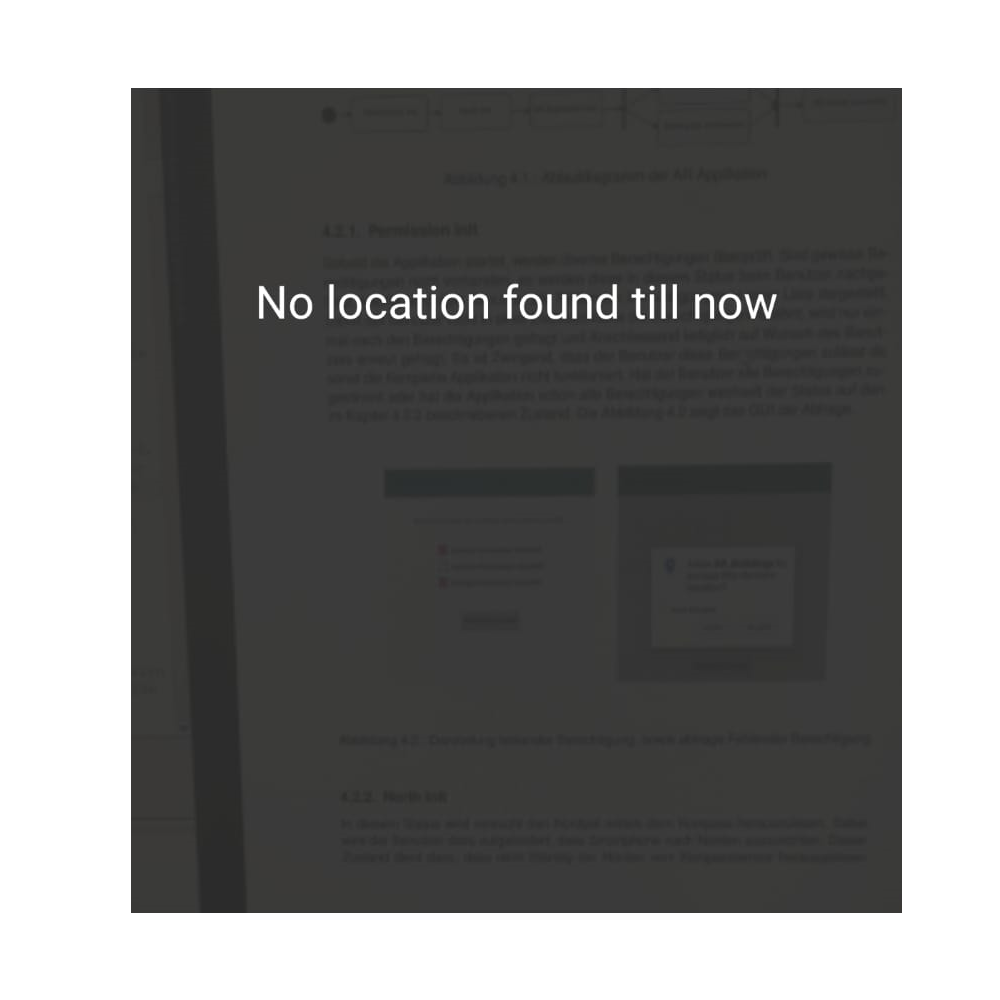
\includegraphics[keepaspectratio, width=\textwidth]{UnknownLocation.png}
	\caption{Darstellung solange Position unbekannt ist.}
    \label{fig:KoordinationNotFound}
\end{figure}


\subsection{3D Model presenting} \label{ch:ThreeDModelPresenting}
In diesem Schritt wird das Model für den Benutzer dargestellt. Das Modell wird mittels eines Gyroscopes stets an der korrekten Stelle gehalten, solange sich der Benutzer an Ort und Stelle hält. Bewegt sich jedoch der Benutzer wieder, werden die neuen Positionsdaten dazu verwendet das Modell darzustellen.
Der Benutzer kann von diesem Zustand wieder in folgende zustände kommen:

\begin{itemize}
	\item North Init (Durch Klicken auf entsprechenden Button siehe Abbildung \ref{fig:ARShowBuilding})
	\item Waiting for localisation (Sofern über eine gewisse Zeit keine neuen Daten hinzugefügt werden konnten).
\end{itemize}

\begin{figure}[h!]
	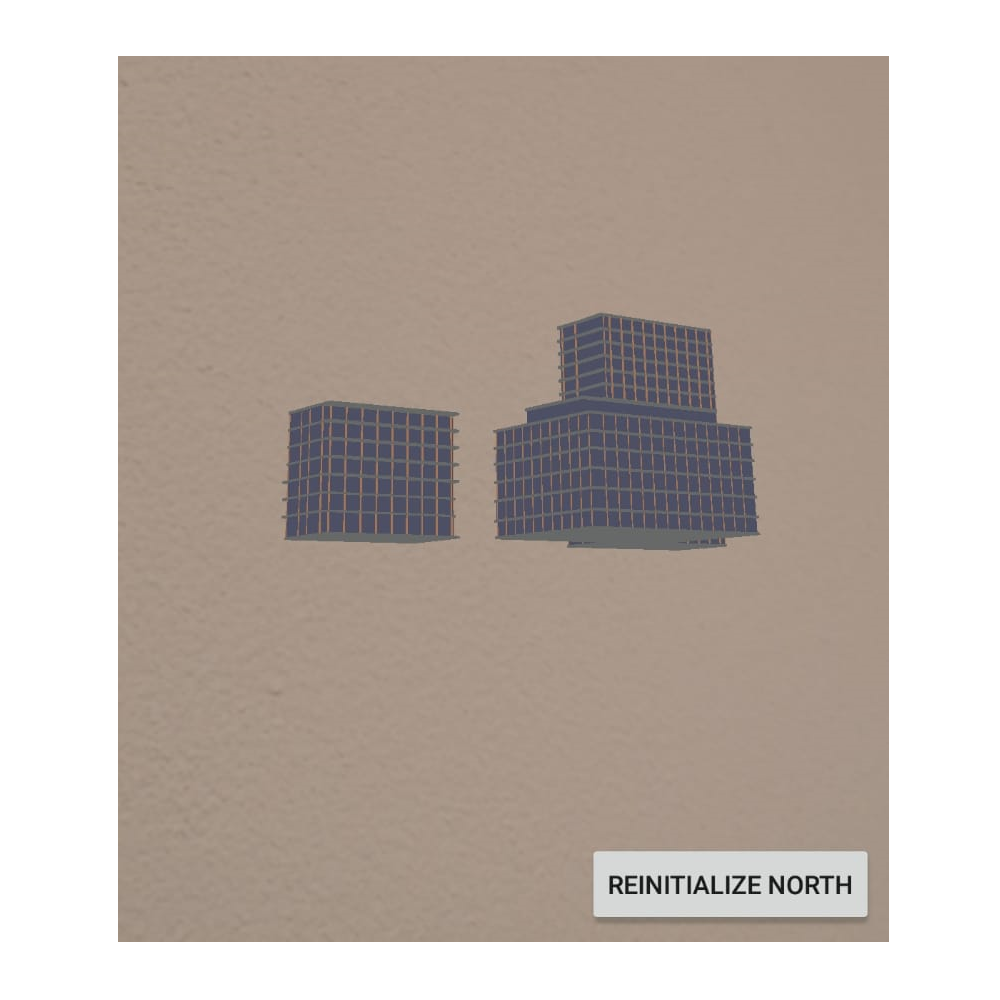
\includegraphics[keepaspectratio, width=\textwidth]{ARShowBuilding.png}
	\caption{Darstellung des Gabäudes sobald die Position ausfindigemacht werden konnte (hier gefälschte Positionsdaten).}
    \label{fig:ARShowBuilding}
\end{figure}

\clearpage

\section{Verworfene Markerbasierte Lösung}
Das Konzept eines markerbasierten Lösung sieht vor, dass die Position des Markers in der realen Welt bereits bekannt ist, und sich diese nicht ändert. Sofern dies der Fall ist, kann die relative Position der Kamera zum Marker und somit zum Gebäude berechnet werden.

Die relative Position zum Marker kann durch dessen Grösse sowie dem Winkel in Relation zur Ausrichtung der Kamera berechnet werden. Sobald diese relative Position berechnet werden konnte, kann die relative Position zum Gebäude ausgerechnet werden.

Der Vorteil dieser markerbasierten Lösung liegt darin, dass die Genauigkeit der Darstellung nicht abhängig von weiteren Faktoren ist. Die grosse Schwäche liegt darin, dass ein Marker zuerst befestigt werden muss, es ist zudem aufwendiger neue Gebäude hinzuzufügen, da man Physisch vor Ort den Marker platzieren muss.

\subsection{Prototyp}
Um dieses Konzept zu Entwickeln wurde ein Prototyp entwickelt. Bei diesem stellte sich jedoch ein schwerwiegendes Problem ein, dass das Gebäude aus nicht weiter untersuchten Gründen beim Gleichen Marker immer wieder verschieden dargestellt wurde. Dieses Verhalten führte dazu, dass die Parallele Entwicklung dieses Konzeptes eingestellt wurde und der Fokus auf die auf der Position basierte Lösung gelegt wurde. In Abbildung \ref{fig:alternativeSolution} sieht man das Fehlverhalten des 3D Modelles.

\begin{figure}[h!]
	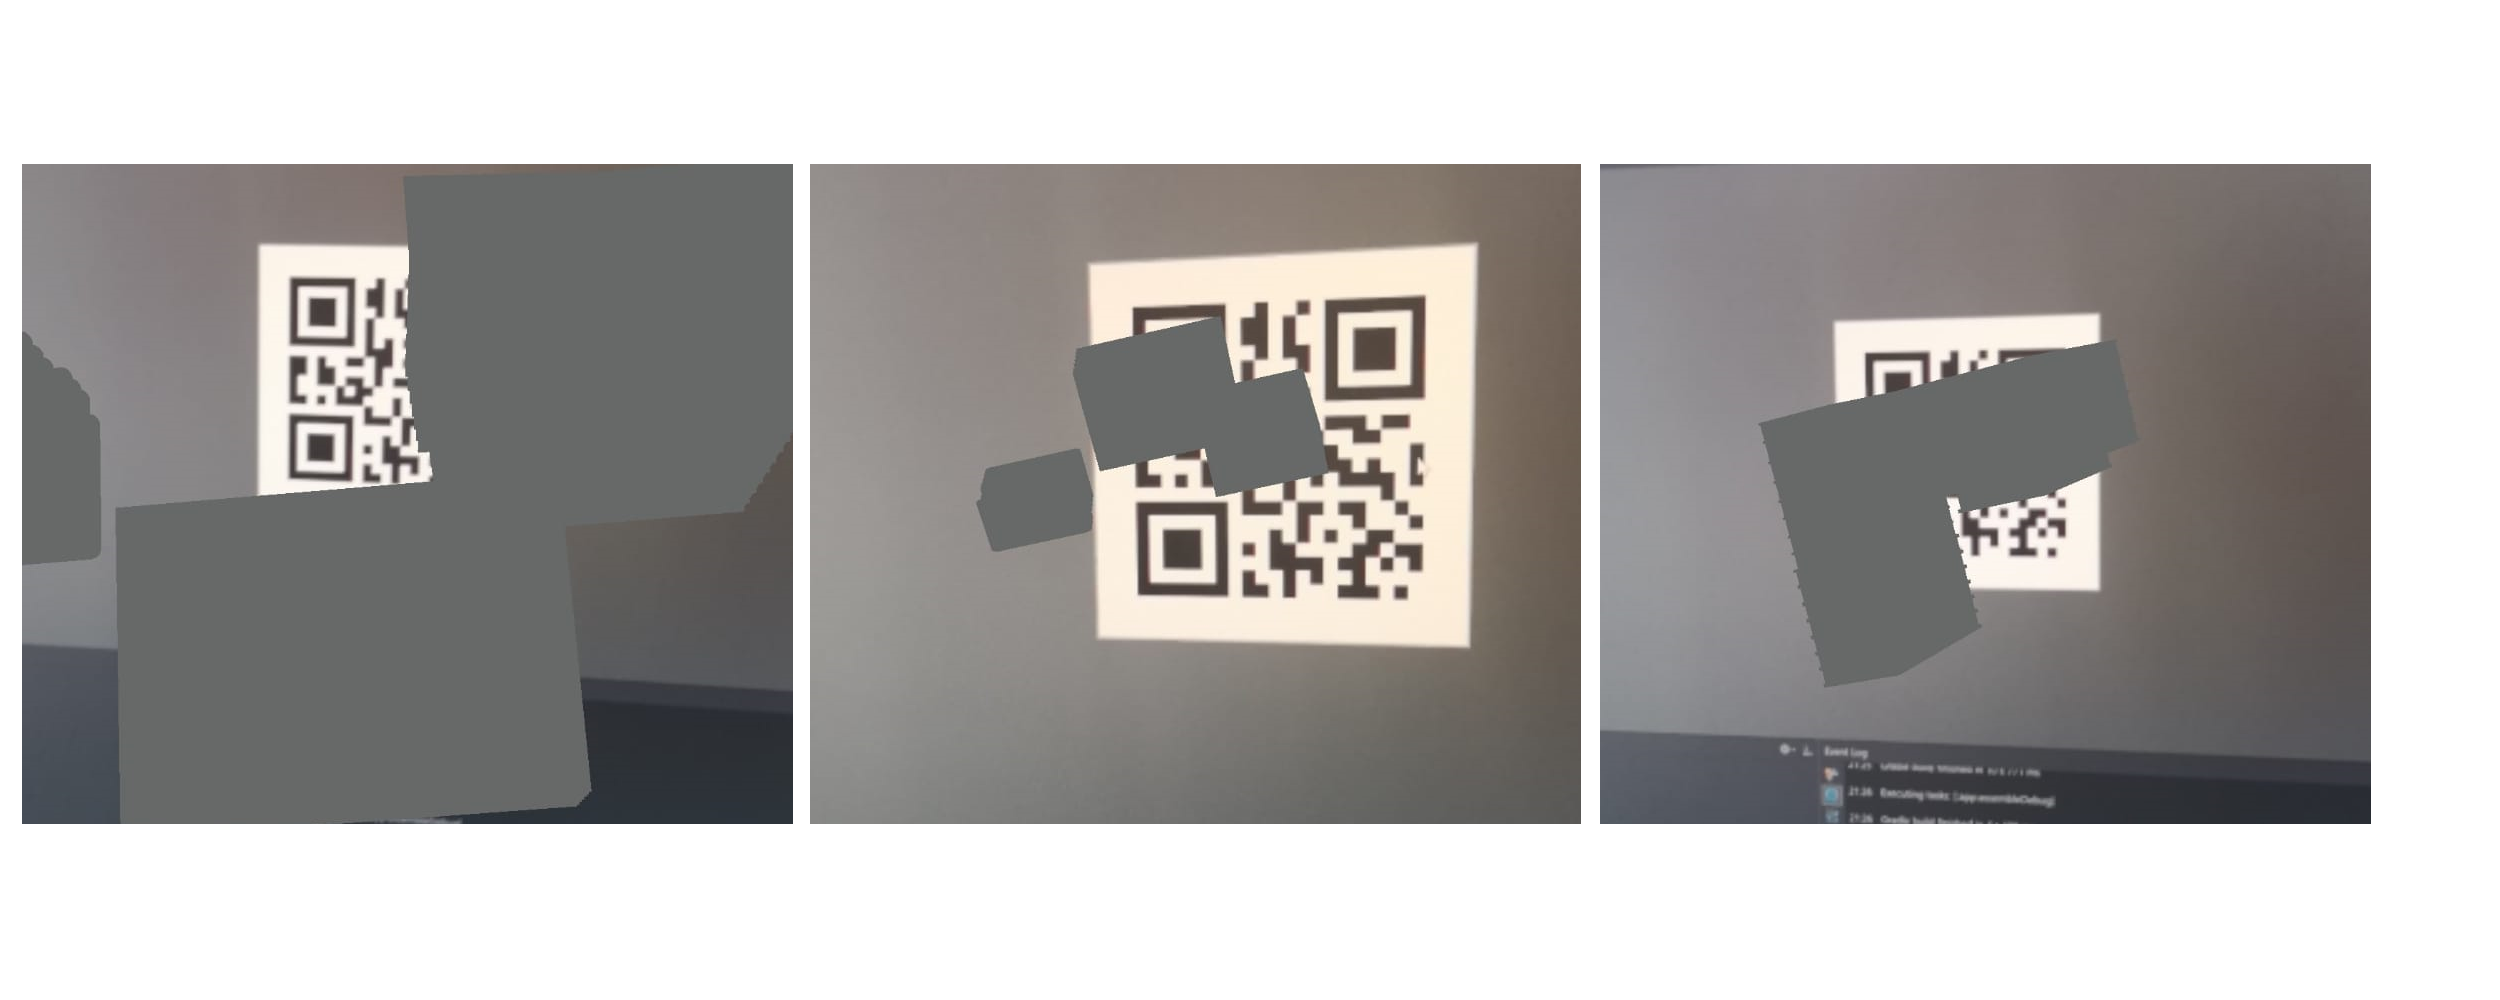
\includegraphics[keepaspectratio, width=\textwidth]{alternativeLoesung.png}
	\caption{Verworfene Alternative Lösung, Problem der unterschiedlichen Darstellungen des Gebäudes.}
    \label{fig:alternativeSolution}
\end{figure}

\chapter{Technische Beschreibung}

\section{Vorgehensmodell}

Alle Wirtschaftsprojekte an der Hochschule Luzern fallen in eine der folgenden Kategorien:

\begin{enumerate}
	\item Einsatz von Standardsoftware und Services
	\item Software- und Produktentwicklung
	\item Innovationsprojekt
	\item IT-Infrastrukturentwicklung
	\item Strukturierte Analyse und Konzeption von Systemen und Abläufen
\end{enumerate}

Dabei ist dieses Projekt als Innovationsprojekt und Softwareentwicklung klassifiziert worden. Wir erwarteten daher unter anderem, eine Evaluation, Recherchen und weitere Unbekannten. Um auf diese eingehen zu können, entschied sich das Team darauf die hybride, inkrementelle Agile Methode zu verwenden.

\subsection{Agile Projektmethode}

Die agile Projektmethode zielt darauf ab in einem ungewissen und sich verändernden Umfeld zu bestehen. Insbesondere heisst das, das auf sich verändernden Voraussetzungen schnell reagiert werden kann und ein funktionierendes Produkt dabei entsteht \parencite{AgileAlliance2015}. Dies soll durch eine enge Zusammenarbeit mit dem Auftraggeber und guter teaminterner Kommunikation erreicht werden.

Ein Rahmenplan dient als Richtschnur des Projektes, während die Anforderungen in den jeweiligen Sprints spezifiziert werden, und in der Sprintplanung festgehalten wird. Wir unterteilten unser Projekt in eine zweiwöchige Initialisierung, zweiwöchige Evaluation, und fünf Sprints, in der unser Produkt entwickelt wurde.

\section{Anforderungen}
\label{ch:Anforderungen}
\begin{itemize}
	\item Das Augmented Reality Objekt soll ausserhalb von Gebäuden ...
	\begin{itemize}
		\item eine maximale Abweichung von 10m auf einer minimalen Distanz von 50m bis zu einer Distanz von 1km auf korrekter Position dargestellt werden (fortan korrekte Position genannt).
		\item eine maximale Rotationsabweichung von \ang{10} aufweisen.
		\item eine maximale Grössenunterschied von 5\% zum Original Aufweisen.
		\item mit einer Maximalen Verzögerung (bei Bewegung) von <1 Sekunde reagieren.
		\item nach Beendigung von langsamen(<=10km/s) Bewegungen der Kamera auf der korrekten Position bleiben.
		\item nach Beendigung von mittelmässig schnellen (>10km/s und <=20km/s) Bewegungen wieder auf korrekter Position dargestellt werden.
		\item nach Beendigungen von schnellen (>20km/s) Bewegungen nach einer erneuten Initialisierung wieder auf korrekter Position dargestellt werden.
		\item nur in einer Distanz bis mindestens 1km dargestellt werden (gilt auch für alle Informationen zum Objekt).
	\end{itemize}
	\item Sobald das Objekt ausserhalb des Sichtfeldes ist, soll dem Benutzer eine Anzeige für das Wiederauffinden des Objektes angezeigt werden.
	\item Sofern keine Informationen zur Lokalisierung vorhanden sind soll der Benutzer in weniger als 3 Sekunden über diese fehlende Informationen informiert werden.
\end{itemize}
\section{Systemspezifikation}
\label{sec:SysSpec}

\subsection{Systemübersicht}

\subsection{Architektur \& Design}
Die Architektur des Projektes wurde in 3 Schichten aufgeteilt. Diese werden in der nachfolgenden Grafik dargestellt.Dabei werden Abhängigkeiten untereinander wie auch zu externen Schnittstellen aufgezeigt.

\begin{figure}[h!]
	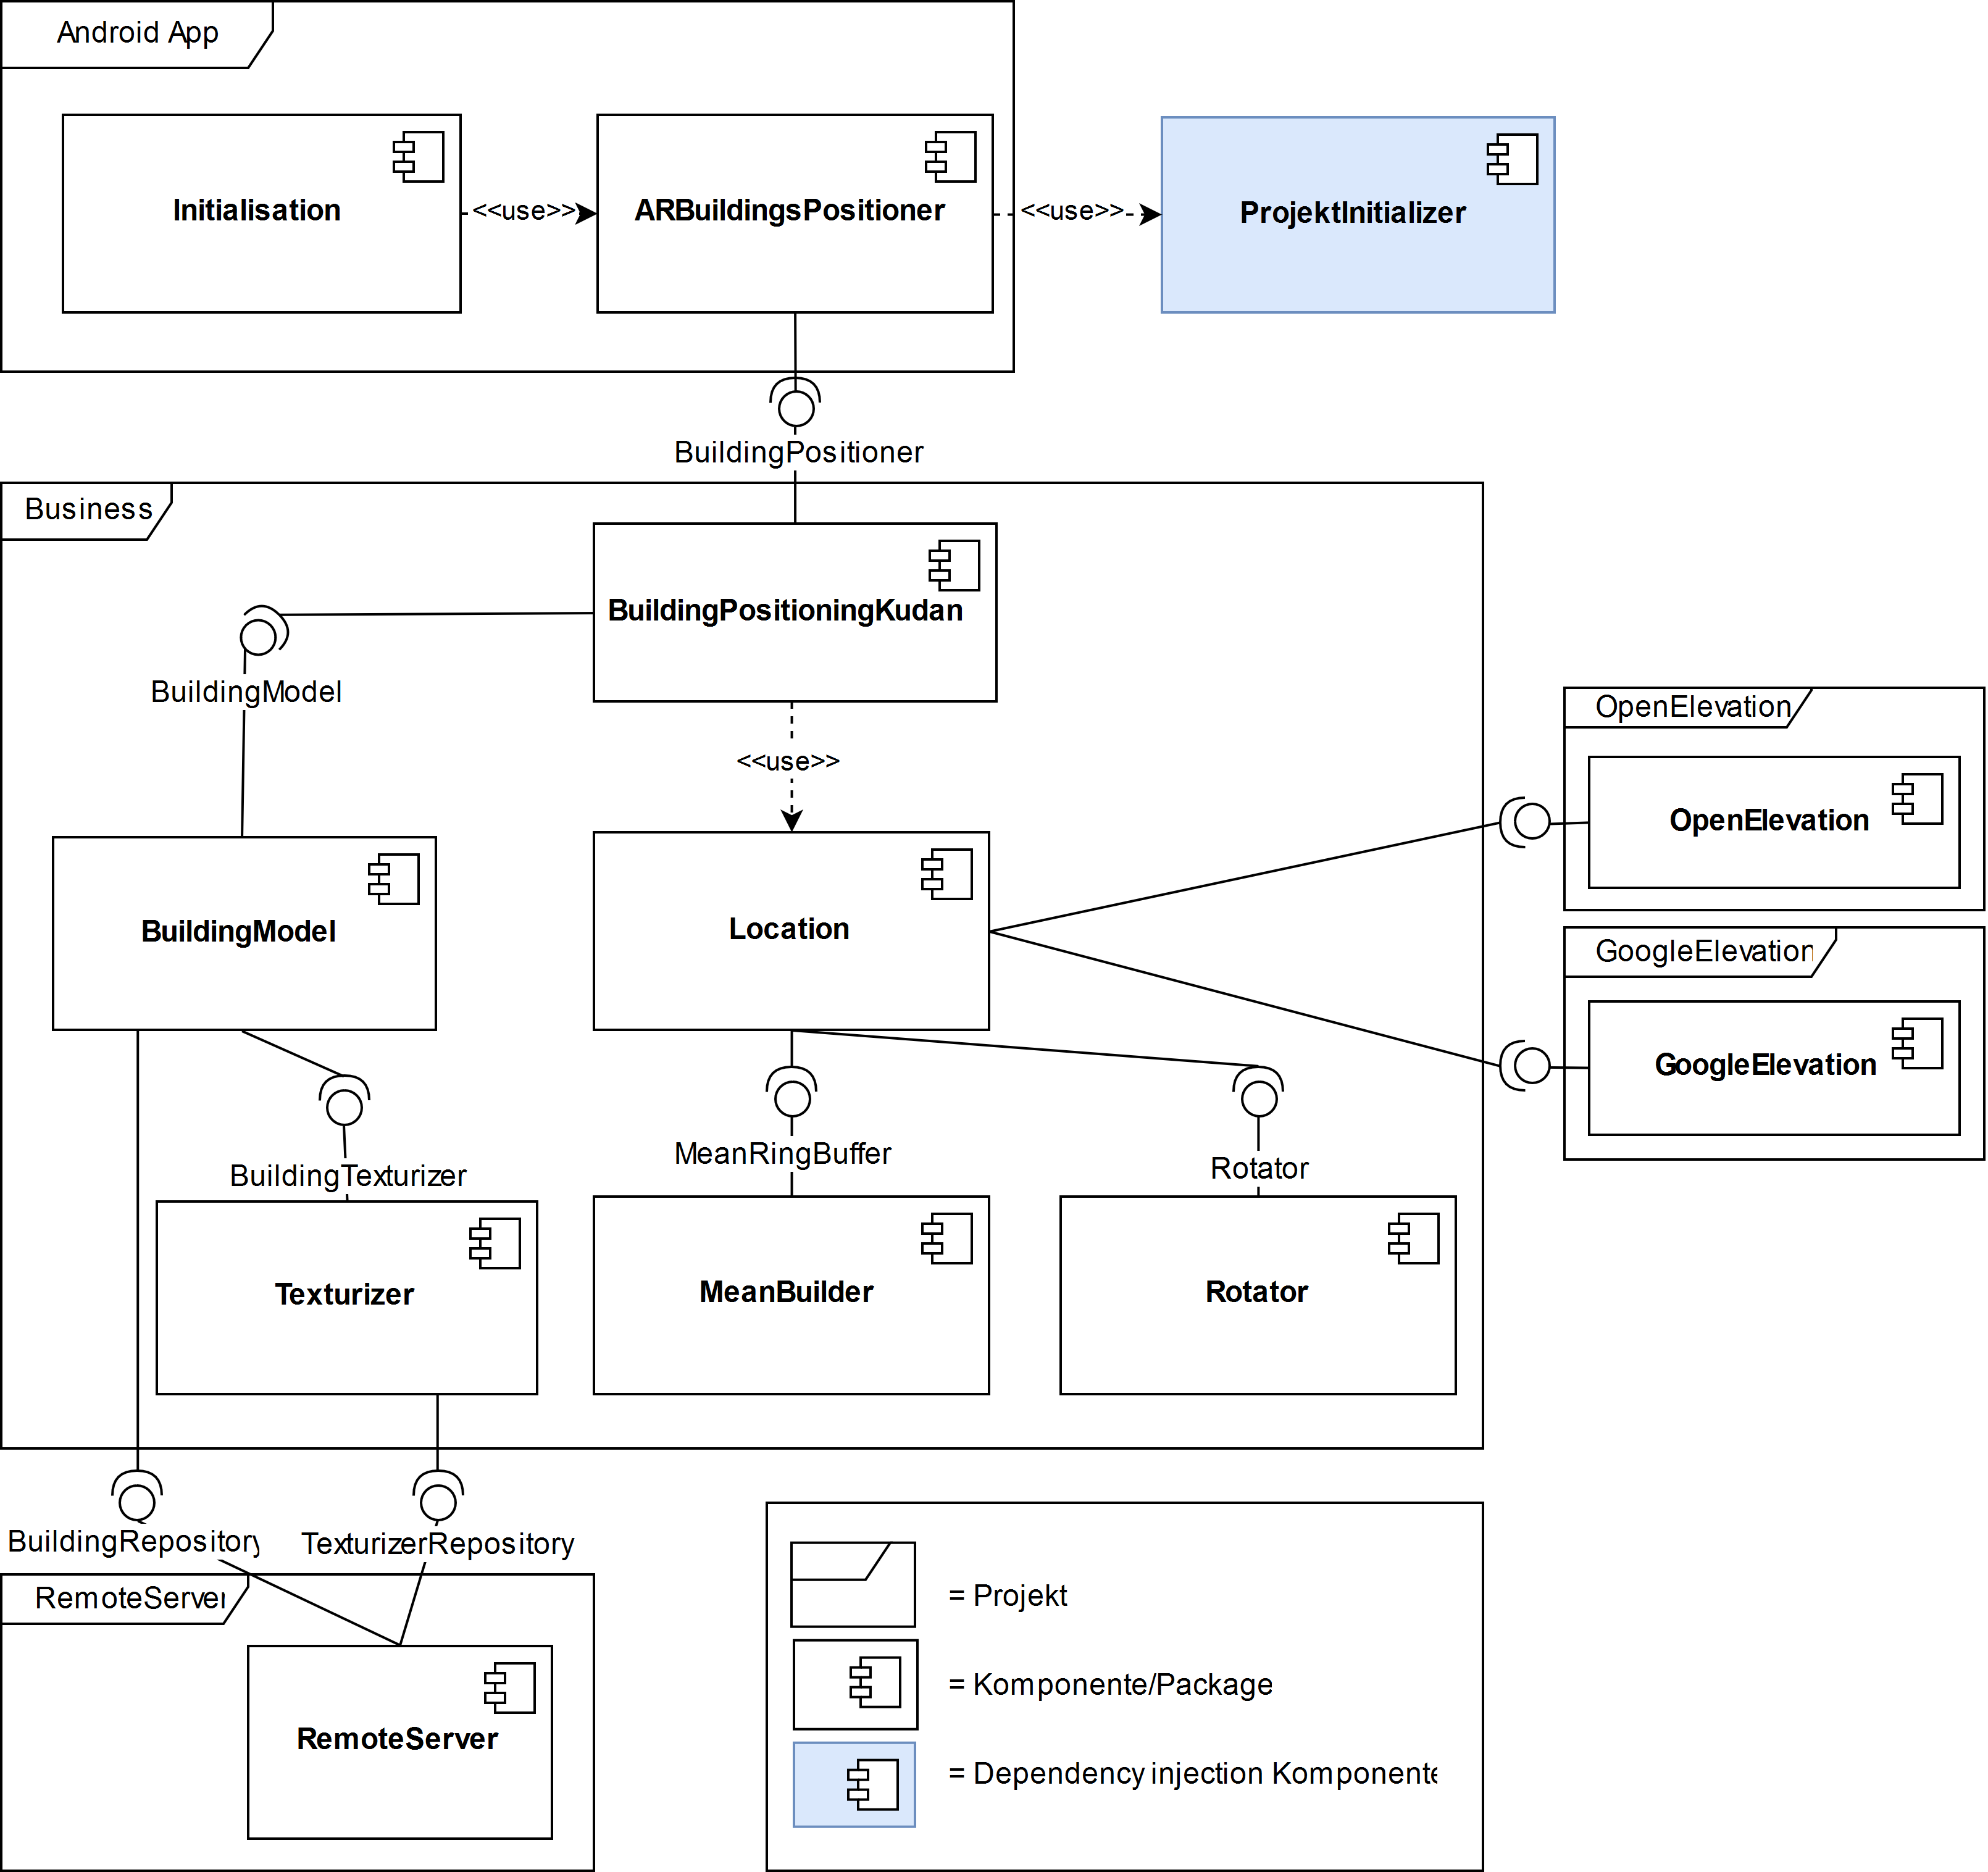
\includegraphics[keepaspectratio, width=\textwidth]{ArchitekturOverviewV0_4.png}
	\caption{Architekturübersicht}
\end{figure}

Eine detaillierte Beschreibung der einzelnen Schichten ist in den folgenden Kapiteln zu finden.

\begin{figure}[h!]
  \center
  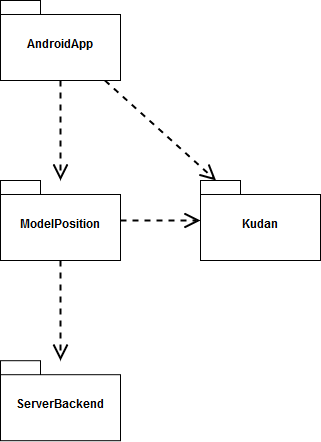
\includegraphics[width=0.35\textwidth]{SchichtenDiagramm.png}
  \caption{Übersicht der simplifizierten Schichtenarchitektur}
\end{figure}

\subsubsection{AndroidApp}
In AndroidApp befindet sich die kompletten grafischen Elemente der Applikation. Dies ist das Interface, mit welchem der User arbeitet. Zudem werden hier die benötigten Berechtigungen geprüft und wenn nötig vom Benutzer erfragt.

\subsubsection{ModelPosition}
In ModelPosition ist die gesamte Logik für die Positionierung eines Gebäudes in der virtuellen Kudan Welt enthalten. Es abstrahiert zudem die Zugriffe auf Kudan selber, sodass diese nicht in der eigentlichen AndroidApp Komponente zu finden sind.

\subsubsection{Server}
Der Server ist eine über eine REST Schnittstelle ansprechbare Komponente, welche das dynamische Laden von neuen Gebäuden ermöglicht. Diese ist ausserhalb dieses Projektscopes, wurde aus Gründen der Vollständigkeit jedoch dokumentiert und spezifiziert.

\subsection{Schnittstellen}
\subsubsection{Externe Schnittstellen}
Neben der Android Bibliothek wurde lediglich KudanAR als externe Schnittstelle verwendet. Die Dokumentation zu dieser Schnittstelle für Android ist unter folgendem Link zu finden:
\href{https://www.kudan.eu/docs-reference/AndroidDocs/annotated.html}{Dokumentation Kudan - Android}


\subsubsection{Interne Schnittstellen}

Die BuildingPositioner Schnittstelle ist verantwortlich für die Abstraktion des gesamten Positionierungsprozesses zur Applikation. Es bietet zudem Methoden an, welche dem Starten und Stoppen des Prozesses dienen.
\begin{figure}[h!]
	\center
	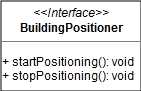
\includegraphics[scale=0.6]{BuildingPositioner.png}
	\caption{BuildingPositioner Interface}
\end{figure}
\clearpage
Das Building Model Interface ist das Bindeglied zwischen der realen Position des Benutzers und der virtuellen Position in der Applikationswelt. Es ist verantwortlich, dass das Gebäude reale Positionsdaten besitzt und die virtuellen Koordinaten an das Modell in der virtuellen Welt übergibt.

\begin{figure}[h!]
	\center
	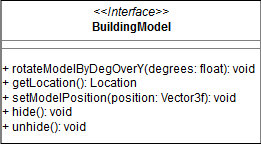
\includegraphics[scale=0.6]{BuildingModel.png}
	\caption{Building Model Interface}
\end{figure}

Der BuildingTexturizer ist verantwortlich für die Einfärbung des Modelles.
\begin{figure}[h!]
	\center
	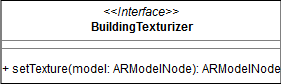
\includegraphics[scale=0.6]{BuildingTexturizer.png}
	\caption{Texturizer Interface}
\end{figure}


Der Rotator verpflichtet sich ein Rotating Object in einem Raum, um eine bestimmte Achse zu drehen.
\begin{figure}[h!]
	\center
	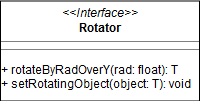
\includegraphics[scale=0.6]{Rotator.png}
	\caption{Rotator Interface}
\end{figure}


Der Mean Ring Buffer ist verantwortlich, dass ein Mittelwert eines Objektes <T> aus den übergebenen Objekten berechnet wird.
\begin{figure}[h!]
	\center
	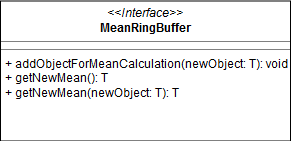
\includegraphics[scale=0.6]{MeanRingBuffer.png}
	\caption{Mean ring buffer Interface}
\end{figure}

Das AsyncElevationRequestCallee abstrahiert die Rückgabemethode für einen AsyncElevationRequest.
\begin{figure}[h!]
	\center
	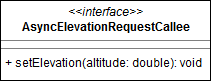
\includegraphics[scale=0.6]{AsyncElevationRequestCallee.png}
	\caption{AsyncElevationRequestCallee Interface}
\end{figure}

\subsection{Anforderungen}

\subsection{Anwendung}

\section{Komponentendesign}

Die Entwickelte Applikation ist von weiteren Kompoenenten und Teilsystemen abhängig. In der Abbildung \ref{fig:Komponentendesign} sind die wichtigsten Komponenten, welche für die Funktionstüchtigkeit notwendig sind abgebildet. Aus Gründen der Übersichtlichkeit sind keine weiteren Komponenten aufgelistet.

Besonderer Augenmerk geht auf die GPS und OpenElevation Komponenten, da diese nicht auf dem Gerät selber sind und daher eine weitere Fehlerquelle (Funktionieren des externen Systems mitbringen).

\begin{figure}[h!]
	\centering
	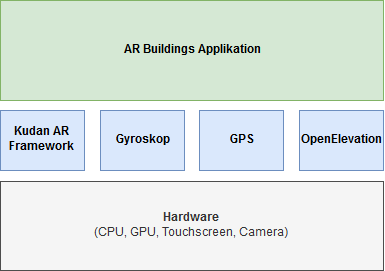
\includegraphics[width=0.7\linewidth, keepaspectratio]{Komponentendesign}
	\caption{Komponenten der ARBuildings Applikation}
	\label{fig:Komponentendesign}
\end{figure}

\section{Umsetzung Programmierung}

\subsection{Clean Code}
Da gut lesbarer Code verständlicher und zeitnaher die Aufgaben des Codes widerspiegelt als ein Kommentar, wurde grösstenteils auf JavaDoc und weitere Kommentare verzichtet. Dieses Verzichten auf zusätzliche Kommentare hatte zur Folge, dass bei der Erstellung einer Methode notwendigerweise ein selbst sprechender Name gewählt werden musste. 

\subsection{Git Flow}
Um möglichst effizient und unabhängig voneinander zu programmieren, sowie zu dokumentieren, wurde mit Git Feature Branch Workflow gearbeitet. Dies bedeutet, dass für jedes Feature einen Branch erstellt worden ist (\cite{gitFeatureBranchWorkflow}). Weiter wurde eine Regelung eingeführt, wobei ein Branch nicht vom Ersteller in den Master Branch zusammengeführt werden darf. Dies schafft Sicherheit, da eine zweite Person einen Review des Codes macht.

\section{Testing}

\subsection{Testfälle}
Basierend auf den Anforderungen, welche in Kapitel \ref{ch:Anforderungen} definiert sind, wurden folgende Tests erstellt. In Kapitel \ref{ch:testprotokoll} ist das Protokoll zu diesen Tests zu finden. Die Testfälle werden mit einer Version versehen. Alte Testfälle sind im git Repository weiterhin verfügbar.

\subsubsection{Testfall 1-Berechtigung erlauben}
\begin{tabularx}{\textwidth}{|l|X|}
\hline 
	Version &
	T-001v1 \\ 
\hline 
	Beschreibung & Berechtigungsanfragen \\ 
\hline 
	Testvoraussetzung & Die App hat die Berechtigungen noch nicht. \\ 
\hline 
	Testschritte &
		1. App starten \\ &
		2. Berechtigungen geben \\
\hline
	Erwartetes Ergebnis & Nachdem alle Berechtigungen gegeben wurden, startet die App normal -> der North Initialize Bildschirm erscheint. \\ 
\hline 
\end{tabularx}
\subsubsection{Testfall 2-Berechtigung verweigern}
\begin{tabularx}{\textwidth}{|l|X|}
\hline 
	Version &
	T-002v1 \\ 
\hline 
	Beschreibung & Berechtigungsanfragen verweigern \\ 
\hline 
	Testvoraussetzung & Die App hat die Berechtigungen noch nicht. \\ 
\hline 
	Testschritte &
		1. App starten \\ &
		2. Berechtigungsanfragen sehen und ablehnen \\
\hline
	Erwartetes Ergebnis & Nachdem alle Berechtigungen nicht gegeben wurden, bleibt die App in einem Abfangbildschirm, wo die Nachfrage für die Berechtigungen erneut gestartet werden kann. \\ 
\hline 
\end{tabularx}
\subsubsection{Testfall 3-Starten von Kudan}
\begin{tabularx}{\textwidth}{|l|X|}
\hline 
	Version &
	T-003v2 \\ 
\hline 
	Beschreibung & 
	Es soll überprüft werden ob die Kudan Komponenten starten.\\ 
\hline 
	Testvoraussetzung &
	T-001 wurde durchgeführt (Berechtigungen erhalten). \\ 
\hline 
	Testschritte &
		1. App starten \\ &
		2. Gerät nach Norden ausrichten \\
\hline
	Erwartetes Ergebnis &
	Es soll der Kamerabildschirm angezeigt werden. \\ 
\hline 
\end{tabularx}
\subsubsection{Testfall 4-Darstellung des Gebäudes Ausrichtung Norden}
\begin{tabularx}{\textwidth}{|l|X|}
\hline 
	Version &
	T-004v2 \\ 
\hline 
	Beschreibung & 
	Bei diesem Testfall soll getestet werden, ob das Gebäude Dargestellt wird.\\ 
\hline 
	Testvoraussetzung &
	Die App ist auf dem Smartphone installiert. GPS gemocked auf folgende Position: \\ & 
		47.145739885261925,8.436641571608824, Altitude: 450 \\ 
\hline 
	Testschritte & 
		1. Smartphone nach Norden ausrichten \\ &
		2. App starten \\ &
		3. Smartphone erneut nach Norden ausrichten \\ &
		4. Initialisierung abwarten (ca. 3 Sekunden)\\
\hline
	Erwartetes Ergebnis &
	Das Gebäude wird auf 7Uhr 30 dargestellt. \\ 
\hline 
\end{tabularx}
\subsubsection{Testfall 5-Darstellung des Gebäudes Ausrichtung Westen}
\begin{tabularx}{\textwidth}{|l|X|}
\hline 
	Version &
	T-005v2 \\ 
\hline 
	Beschreibung & 
	Bei diesem Testfall soll getestet werden, ob das Gebäude dargestellt wird, wenn es nicht nach norden gerichtet ist. \\ 
\hline 
	Testvoraussetzung &
	Die App ist auf dem Smartphone installiert. GPS gemocked auf folgende Position: \\ &
		47.145739885261925,8.436641571608824, Altitude: 450 \\ 
\hline 
	Testschritte & 
		1. Smartphone nach Westen ausrichten \\ &
		2. App starten \\ &
		3. Smartphone nach Norden ausrichten \\
\hline
	Erwartetes Ergebnis &
	Das Gebäude wird auf 7Uhr 30 dargestellt. \\ 
\hline 
\end{tabularx}
\subsubsection{Testfall 6-Darstellung Gebäude mit Bewegung nach rechts}
\begin{tabularx}{\textwidth}{|l|X|}
\hline 
	Version &
	T-006v2 \\ 
\hline 
	Beschreibung & 
	Bei diesem Testfall soll getestet werden, ob das Gebäude dargestellt wird und sich die Position des Gebäudes den GPS Daten anpasst. \\ 
\hline 
	Testvoraussetzung &
	Die App ist auf dem Smartphone installiert. GPS gemocked auf folgende Position: \\ &
		47.145739885261925,8.436641571608824, Altitude: 450 \\ 
\hline 
	Testschritte & 
		1. Smartphone nach Westen ausrichten \\ &
		2. App starten \\ &
		3. Smartphone nach Norden ausrichten \\ &
		4. App minimieren (Home Button drücken) \\ &
		5. GPS Mocklocation verändern (auf Position 47.145739885261925,8.436641571608824) \\ &
		6. App erneut öffnen \\
\hline
	Erwartetes Ergebnis &
	Das Gebäude wandert von 7Uhr 30 auf 9Uhr \\ 
\hline 
\end{tabularx}
\subsubsection{Testfall 7-Darstellung Gebäude mit Bewegung nach links}
\begin{tabularx}{\textwidth}{|l|X|}
\hline 
	Version &
	T-007v2 \\ 
\hline 
	Beschreibung & 
	Bei diesem Testfall soll getestet werden, ob das Gebäude dargestellt wird und sich die Position des Gebäudes den GPS Daten anpasst. \\ 
\hline 
	Testvoraussetzung &
	Die App ist auf dem Smartphone installiert. GPS gemocked auf folgende Position: \\ &
		47.142958, 8.430126, Altitude: 450 \\ 
\hline 
	Testschritte & 
		1. Smartphone nach Norden ausrichten \\ &
		2. App starten \\ &
		3. Smartphone nach Norden ausrichten \\ &
		4. App minimieren (Home Button drücken) \\ &
		5. GPS Mocklocation verändern (auf Position  47.141427, 8.432621) \\ &
		6. App erneut öffnen \\
\hline
	Erwartetes Ergebnis &
	Das Gebäude wandert von 15Uhr auf 12Uhr \\ 
\hline 
\end{tabularx}
\subsubsection{Testfall 8-Entfernen der Berechtigung zur Laufzeit}
\begin{tabularx}{\textwidth}{|l|X|}
\hline 
	Version &
	T-008v1 \\ 
\hline 
	Beschreibung & 
	Bei diesem Testfall so überprüft werden ob die App nicht abstürzt, wenn zur Laufzeit der App Berechtigungen entzogen werden. \\ 
\hline 
	Testvoraussetzung &
	Die App ist auf dem Smartphone installiert und hat alle nötigen Berechtigungen \\ 
\hline 
	Testschritte & 
		1. App starten \\ &
		2. App minimieren \\ &
		3. Berechtigungen der App entfernen \\ &
		4. App wieder öffnen \\
\hline
	Erwartetes Ergebnis &
	Die App schaltet wieder auf den Berechtigungsbildschirm. \\ 
\hline 
\end{tabularx}
\subsubsection{Testfall 9-Smartphone Rotation}
\begin{tabularx}{\textwidth}{|l|X|}
\hline 
	Version &
	T-009v2 \\ 
\hline 
	Beschreibung & 
	Es soll überprüft werden wie das Verhalten ist, wenn das Smartphone rotiert wird. \\ 
\hline 
	Testvoraussetzung &
	Die App hat alle Berechtigungen \\ 
\hline 
	Testschritte & 
		1. App starten \\ &
		3. Smartphone nach Norden ausrichten \\ &
		3. Rotieren des Smartphones um 90 Grad (Portrait auf Landscape) \\
\hline
	Erwartetes Ergebnis &
	Die App soll keine Rotationsanimation beinhalten. Die App soll das Gebäude weiter anzeigen. \\ 
\hline 
\end{tabularx}
\subsubsection{Testfall 10-Spezialtest Überprüfung mittels Gebäude}
\begin{tabularx}{\textwidth}{|l|X|}
\hline 
	Version &
	T-010v1 \\ 
\hline 
	Beschreibung & 
	Es soll überprüft werden, ob das Bestehende Gebäude mit dem AR Gebäude Deckungsgleich ist.\\ 
\hline 
	Testvoraussetzung &
	Die App hat alle Berechtigungen \\ &
	Teil des Gebäudekomplex ist Sichtbar\\ &
	Der Tester befindet sich vor Ort\\ 
\hline 
	Testschritte & 
		1. Tester läuft auf Position (47.142835, 8.431436) \\ &
		2. App starten \\ &
		3. Smartphone nach Norden ausrichten \\ &
		4. Gebäudekomplex in Kamera fokussieren. \\
\hline
	Erwartetes Ergebnis &
	Die App soll das AR Modell über dem Realen Gebäude darstellen. \\ &
	Randbedingungen: \\ &
		Maximale Abweichung 10m in alle Richtungen.\\ 
\hline 
\end{tabularx}

\subsection{Testprotokoll}
\label{ch:testprotokoll}
Die Folgende Tabelle Zeigt ob die Tests erfolgreich waren oder nicht. Genauere Resultate sind im Anhang \ref{appendig:testprotokolle} zu finden . 
\bigbreak

\begin{tabularx}{\textwidth}{|l|X|l|}
\hline
	\textbf{TestID/Version }& \textbf{Beschreibung} & \textbf{Passed} \\
\hline
	T-001v1 & Berechtigungsanfragen & \checkmark \\
\hline
	T-002v1 & Berechtigungsanfragen verweigern & \checkmark \\
\hline
	T-003v2 & Es soll überprüft werden ob die Kudan Komponenten starten. & \checkmark \\
\hline
	T-004v2 & Bei diesem Testfall soll getestet werden, ob das Gebäude Dargestellt wird. & \checkmark \\
\hline
	T-005v2 & Bei diesem Testfall soll getestet werden, ob das Gebäude dargestellt wird, wenn es nicht nach norden gerichtet ist. & \checkmark \\
\hline
	T-006v2 & Bei diesem Testfall soll getestet werden, ob das Gebäude dargestellt wird und sich die Position des Gebäudes den GPS Daten anpasst. & \checkmark \\
\hline
	T-007v2 & Bei diesem Testfall soll getestet werden, ob das Gebäude dargestellt wird und sich die Position des Gebäudes den GPS Daten anpasst. & \checkmark \\
\hline
	T-008v1 & Bei diesem Testfall so überprüft werden ob die App nicht abstürzt, wenn zur Laufzeit der App Berechtigungen entzogen werden. & \checkmark \\
\hline
	T-009v2 & Es soll überprüft werden wie das Verhalten ist, wenn das Smartphone rotiert wird. & \checkmark \\
\hline
\end{tabularx}

\chapter{Realisierung}

% TODO Ein Beispiel für den Gebrauch von Formeln und Referenz auf die jeweilige Formel - entfernen wenn nicht mehr gebraucht
Die Distanz zwischen zwei Geopositionen wird über die Bogenlänge (siehe \ref{Bogenlaenge}) der Differenz der Längen- und Breitengrade ausgerechnet.

\indexequation{b = \frac{\pi}{\SI{180}{\degree}}\beta r}{Bogenlänge des Winkels $\beta$ mit Radius $r$}{Bogenlaenge}

\section{Ermittlung offener Projektrahmenbedingungen}
\label{sec:evaluation}
Im Rahmen dieses Projektes mussten verschiedene Unbekannte zuerst analysiert und evaluiert werden. Dazu gehörten die Zielplattform, Entwicklungsumgebung und die zu verwendenden Augmented Reality Frameworks.
\subsubsection{Zielplattform}
Als Zielplattform standen gemäss Projektbeschrieb die Folgenden zur Auswahl:
\begin{itemize}
\item Microsoft HoloLens
\item Smartphone und Tablets
\end{itemize}
Für alle dieser Plattformen galt die Idee, diese als Interface zu gebrauchen um das AR Gebäude in der Umgebung anzuzeigen. Alle drei Zielplattformen weisen unterschiedliche Stärken und Schwächen auf.


Die HoloLens zeigte grosse Schwächen beim Gebrauch im Freien, da deren Bildschirm für den Aussengebrauch zu wenig Hell ist.

Zudem fehlen der HoloLens Lokalisierungssensoren. Im Rahmen einer Analyse der Bedienung wurden 5 Probanden dazu aufgefordert mit der vorhanden HoloLens und HoloLens Apps zu interagieren, und ihr Verhalten beobachtet. Die Probanden besassen keinerlei Erfahrung im Umgang mit der HoloLens und es wurde ihnen auch keine vorgängigen Informationen zur Bedienung mitgeteilt. Bei diesem Test stellte sich heraus, dass die Interaktion mit der HoloLens für alle Probanden nicht intuitiv war. Dies äusserte sich in Gesten, die von der HoloLens nur manchmal erkannt wurden (Pinching) und solche die zwar für Probanden intuitiv waren, aber von der Hololens ignoriert wurden (antippen eines virtuellen Objektes).
Das Positive der HoloLens ist die nahtlose Integration der Augmented Reality Modelle in die Umgebung des Betrachters. 
 
Die Smartphones zeigen ihre grosse Stärke in der Verbreitung. Dies führt zu einer hohen Vertrautheit des Benutzers mit dem Gerät. Zudem sind die heutigen Smartphones hell genug um das Display bei normalen Tageslicht zu sehen.
Nachteile zeigen sich in der Haltung des Gerätes, da für die Einbindung der Augmented Reality Modelle das Smartphone ständig in den Händen gehalten werden muss.

In einer ersten Evaluation mit einer Hololens wurde entschieden, dass für dieses Projekt die Hololens ausgeschlossen werden soll, da diese für Ausseneinsätze nur bedingt verwendet werden kann.

Dank der höheren Verbreitung und der damit entstehenden höheren Flexibilität beim Entwickeln, fiel die Entscheidung auf eine Lösung für Smartphones. Es wurde schliesslich noch auf die Android Plattform eingeschränkt, dies aus den Gründen, dass Android keine speziellen Bedingungen voraussetzt und somit auch auf den bereits vorhanden Geräten verwendet werden kann. 

\subsubsection{Entwicklungsumgebung}
\label{ssec:EvalPlattform}
Bedingt durch die Selektion der Zielplatform standen verschiedene Entwicklungsumgebungen zur Verfügung. Dabei wurden folgende zwei Entwicklungsumgebungen miteinander verglichen:
\begin{itemize}
\item Unity
\item AndroidStudio
\end{itemize}

Auf beiden Entwicklungsumgebungen wurde ein Prototyp für Android entwickelt. Dabei entstand folgende Auffassung:

Bei Unity ist das Erstellen einer ersten lauffähigen Version sehr einfach. Ein weiterer Vorteil ist die grafische Darstellung der 3D Modelle. Zudem würde eine allfällige Portierung auf weitere Platformen einfach umsetzbar sein. Bei der Entwicklung stellte sich eine Schwäche mit den GPS Sensoren heraus. So funktionierten diese aus unbekannten Gründen nicht bei jeder Installation der Applikation korrekt. Für die Lösung dieses Problemes fehlte eine ausreichende Debugmöglichkeit in Unity.

Android Studio zeigte seine Stärke in den Debugmöglichkeiten und der ausgezeichneten API Dokumentation. So funktionierten alle benötigten Sensoren auf Anhieb. Die Schwächen dieser Entwicklungsumgebung liegt darin, dass eine allfällige Portierung auf weitere Plattformen nur durch eine Neuimplementation möglich ist. Zudem werden die 3D Modelle nicht grafisch dargestellt und müssen mit einer anderen Software Editiert werden.

Die unzureichende Debugmöglichkeiten sowie die Problemen mit den GPS Sensoren waren die Hauptgründe die Unity Entwicklungsumgebung nicht für die Implementation zu gebrauchen.

\subsubsection{Augmented Reality Frameworks}
Während der Recherchen stellte sich heraus, dass ein breites Spektrum verschiedener AR Frameworks auf dem Markt vorhanden ist. Jedes Framework setzt dabei auf eigene Anwendungsbereiche. Für dieses Projekt wurden vier häufig verwendete und gut dokumentierte Frameworks näher untersucht (\cite{DDIDevelopment}). Konkret handelte es sich dabei um folgende Frameworks:
\begin{itemize}
\item Kudan
\item Vuforia
\item Wikitude
\item ARtoolKit
\end{itemize}

Die Folgende Tabelle zeigt eine vereinfachte Darstellung der 4 Frameworks. Sie vergleicht die für dieses Projekt notwendigen Features, sowie die Lizenzierung (\cite{DDIDevelopment}).

\begin{table}[h!]
	\center
	\begin{tabular}{|c|c|c|c|c|}
		\hline 
		& \textbf{Mobile} & \textbf{UWP (Hololens)} & \textbf{SLAM} & \textbf{Licence} \\ 
		\hline 
		Kudan & \checkmark & x & \checkmark & Commercial, free \\ 
		\hline 
		Vuforia & \checkmark & \checkmark & \checkmark & Commercial \\ 
		\hline 
		Wikitude & \checkmark & \checkmark & \checkmark & Commercial, free \ \\ 
		\hline 
		ARToolkit & \checkmark & x & x & OpenSource \\ 
		\hline 
	\end{tabular}
	\caption{Vergleichstabelle verschiedener AR Frameworks}
\end{table}


Für das Projekt wurde entschieden Kudan als AR Framework zu verwenden. Gründe dafür lagen darin, dass dieses Framework über eine sehr robuste single-Kamera SLAM Implementation verfügt (\cite{BerfinAyhan2017}), und das Lizenzierungsmodell, welche eine Entwicklung ohne weitere Kosten ermöglichte. Der wichtigste Grund lag jedoch darin, dass die Dokumentation sehr extensiv, und die Erfahrung mit Kudan am Grössten war.

\section{Einschränkungen und Abgrenzungen}

Wie aus der Evaluation (siehe \ref{ssec:EvalPlattform}) ersichtlich ist, haben wir uns schlussendlich auf Android als Plattform beschränkt. Dies hat zur Folge, dass der erarbeitete Code nicht ohne weiteres auf andere Plattformen portiert werden kann. Die Architektur ist aber so modular aufgebaut, dass die Implementierung für andere Plattformen dennoch ohne grossen Aufwand geschehen kann.

Weiter haben wir die Androidversion auf Version 6.0 und aufwärts eingeschränkt. Dies entspricht etwa 80\% aller Androidbesitzer (siehe Abb. \ref{fig:AndroidMarketshare}), und beinhaltet wichtige Funktionen die wir für unser Projekt gebrauchen. Zudem muss das jeweilige Gerät folgende Systemanforderungen besitzen:
\begin{itemize}
	\item Gyroskop
	\item Magnetometer (Kompass)
	\item GPS Lokationssensor (GLOSNASS, GALILEO, BEIDU)
\end{itemize}

\begin{figure}
	\centering
	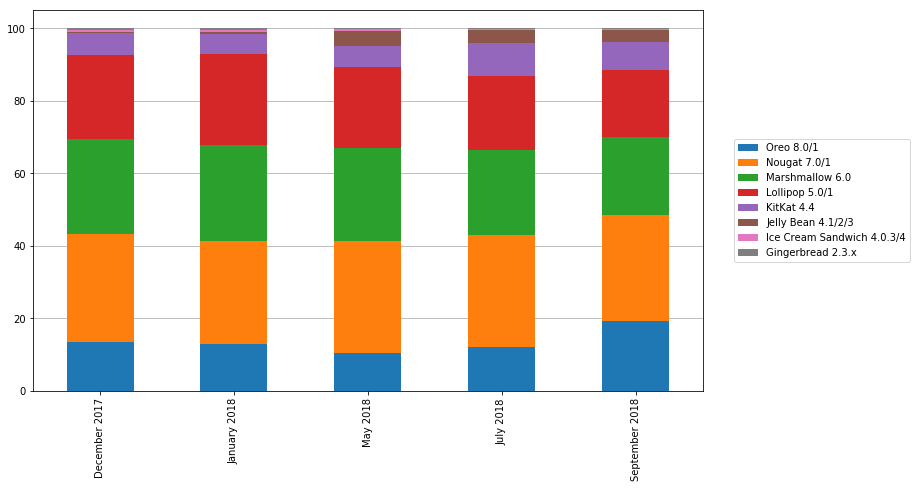
\includegraphics[keepaspectratio,width=0.8\textwidth]{AndroidMarketshare}
	\caption{Prozentanteil der Androidversionen, Daten von \cite{Fossbytes2018}}
	\label{fig:AndroidMarketshare}
\end{figure}


\newpage
\section{Projektmanagementplan}

\subsection{Projektorganisation}
Da beide Projektmitglieder ihre Kompetenzen eher in den technischen Bereichen dieses Projekts sehen, wurde von einer strikten Aufgabenteilung abgesehen.

Es wurde dennoch darauf geachtet, dass beide Mitglieder klare Verantwortungen übernehmen. Diese waren jedoch mehr in einer überwachenden Funktion gesehen, und soll nicht heissen, dass dieses Mitglied die Arbeit alleine leistete.

\vspace{1em}

\begin{tabularx}{\textwidth}{|X|X|}
	\hline
	\textbf{Teammitglied} & \textbf{Funktionen} \\
	\hline
	Pascal Baumann & \tabitem Dokumentation \\
	& \tabitem Testplanung \& Durchführung \\
	& \tabitem Projektmanagement \\
	\hline
	Dane Wicki & \tabitem Architektur \\
	& \tabitem Plattformanalyse \\
	\hline
\end{tabularx}

\newpage
\subsection{Projektführung}

\subsection{Rahmenplan}

Das Projekt wurde in 6 zweiwöchige Sprints unterteilt und in diesen iterativ entwickelt.

\vspace{1em}

\begin{figure}[h!]
	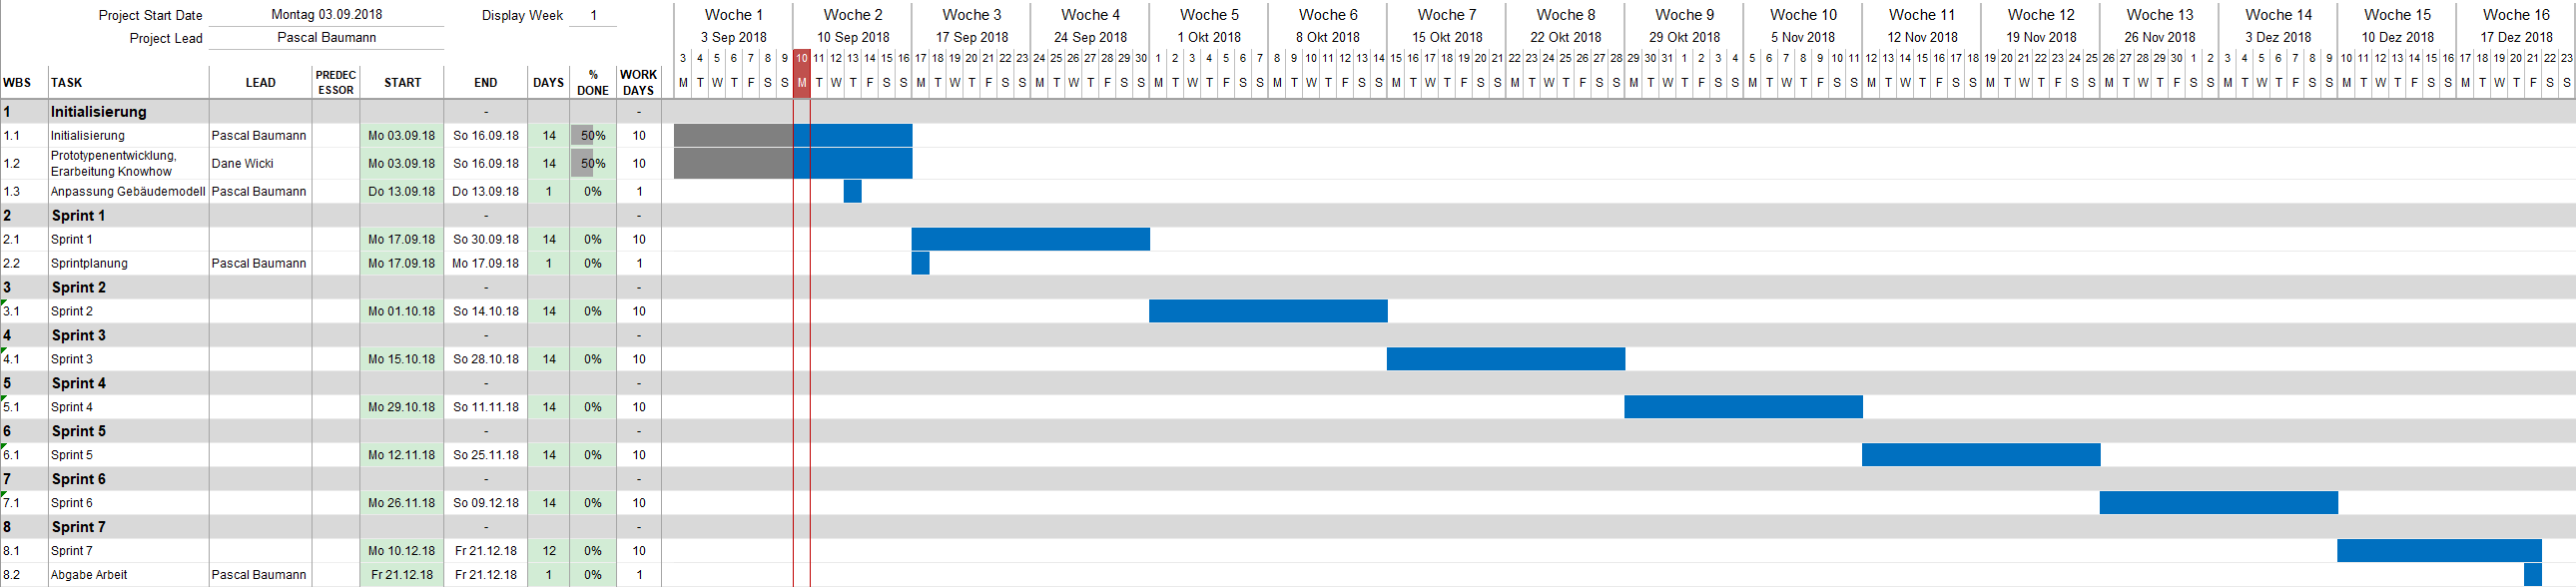
\includegraphics[keepaspectratio, width=\textwidth]{Rahmenplan}
	\caption{Überblick der Sprints}
\end{figure}

\subsection{Tools}
\label{sec:Tools}
\begin{table}[h!]
	\begin{tabular}{|p{0.4\textwidth}|p{0.6\textwidth}|}
		\hline
		\textbf{Aufgabe} & \textbf{Hilfsmittel} \\
		\hline
		Dokumente und Dokumentation & TeX / GitHub \\
		\hline
		Versionierung Dokumentation & git / GitHub\\
		\hline
		Dokumentation Code & JavaDoc \\
		\hline
		Git Clients & GitKraken, git Terminal\\
		\hline
		Quellen & Mendeley \\
		\hline
		Dateiablage für Teamaustausch & OneDrive \\
		\hline
		Rahmenplan & MS Excel 2016 \\
		\hline
		Kommunikation Team & WhatsApp\\
		\hline
		Aufgabenverwaltung & Trello, Rahmenplan\\
		\hline
		Entwicklungsumgebung Arduino & Arduino Studio\\
		\hline
	\end{tabular}
	\caption{Gebrauchte Software Hilfsmittel}
	\label{tab:SWTools}
\end{table}

\subsection{Risikomanagement}

Es werden mögliche Risiken, welche während dem Projekt auftreten können aufgezählt. Diese werden auf Eintrittswahrscheinlichkeit und Schadensmass eingeschätzt, danach wird entschieden, welche Massnahmen getroffen werden können, und was deren Auswirkungen sind.

\subsubsection{Definitionen}
\label{sssec:Def}
\vspace{1em}
\noindent
Eintrittswahrscheinlichkeit:

\vspace{1em}
\noindent
\begin{tabular}{|p{0.06\textwidth}|p{0.2\textwidth}|p{0.7\textwidth}|}
	\hline
	\textbf{Stufe} & \textbf{Bezeichnung} & \textbf{Beschreibung} \\
	\hline
	1 & unvorstellbar & Möglich aber eher unwahrscheinlich. Tritt nie oder einmal in 14 Wochen auf \\
	\hline
	2 & unwahrscheinlich & Kann in 14 Wochen 1-5 Mal eintreten\\
	\hline
	3 & vorstellbar & Kann in 14 Wochen 6-8 Mal eintreten \\
	\hline
	4 & wahrscheinlich & Kann in 14 Wochen bis zu 10 Mal eintreten \\
	\hline
	5 & häufig & Kann in 14 Wochen 14 Mal eintreten\\
	\hline
\end{tabular}

\vspace{1em}
\noindent
Schadensausmass:

\vspace{1em}
\noindent
\begin{tabular}{|p{0.06\textwidth}|p{0.2\textwidth}|p{0.7\textwidth}|}
	\hline
	\textbf{Stufe} & \textbf{Bezeichnung} & \textbf{Beschreibung} \\
	\hline
	1 & unwesentlich & Die Aufgabenerfüllung wird höchstens geringfügig beeinträchtigt, finanzieller Schaden ist im Rahmen des Projekts nicht beeinflussend. Personenschäden treten nicht auf \\
	\hline
	2 & geringfügig & Wahrnehmbare Gefährdung / Einfluss auf das Projekt. Personenschäden treten nicht auf \\
	\hline
	3 & mittelmässig & Wahrnehmbare Gefährdung / Einfluss auf das Projekt.Finanzieller Schaden strapaziert das Projektbudget
	Personenschäden treten nicht auf \\
	\hline
	4 & kritisch & Starke Gefährdung des Projekts. Finanzieller Schaden übersteigt das Projektbudget massiv. Personenschäden treten geringfügig auf.\\
	\hline
	5 & katastrophal & Projektabbruch zur Folge. Finanzieller Schaden kann zum Projektstopp führen. Verletzung der Persönlichkeitsrechte.
	\\
	\hline
\end{tabular}

\subsubsection{Risikokatalog}
\label{sssec:Risikokatalog}
Legende:
\begin{itemize}
	\item \textbf{S}chadensausmass bei Eintreffen des Risikos
	\item \textbf{W}ahrscheinlichkeit das Risiko eintrifft
	\item \textbf{K}ategorie: \textbf{T}echnisches oder \textbf{P}rojektbezogenes Risiko
	\item \textbf{A}uswirkung auf das Projekt. Produkt aus S und W
\end{itemize}

\vspace{1em}
\noindent
\begin{tabular}{|p{0.03\textwidth}|p{0.75\textwidth}|p{0.03\textwidth}|p{0.03\textwidth}|p{0.03\textwidth}||p{0.03\textwidth}|}
	\hline
	\textbf{Nr.} & \textbf{Beschreibung / Risiko} & \textbf{K} & \textbf{S} & \textbf{W} & \textbf{A} \\
	\hline
	1 & Datenverlust & P & 5 & 1 & 5\\
	\hline
	2 & Fehlkommunikation im Team & P & 3 & 2 & 6 \\
	\hline
	3 & Teammitglied fällt aus & P & 3 & 2 & 6 \\
	\hline
	4 & Verzug bei Erstellung von Dokumenten & P & 3 & 2 & 6 \\
	\hline
	5 & Prototyp entspricht nicht den Kundenwünschen & T & 5 & 2 & 10 \\
	\hline
\end{tabular}

\vspace{1em}

\begin{figure}[h!]
	\centering
	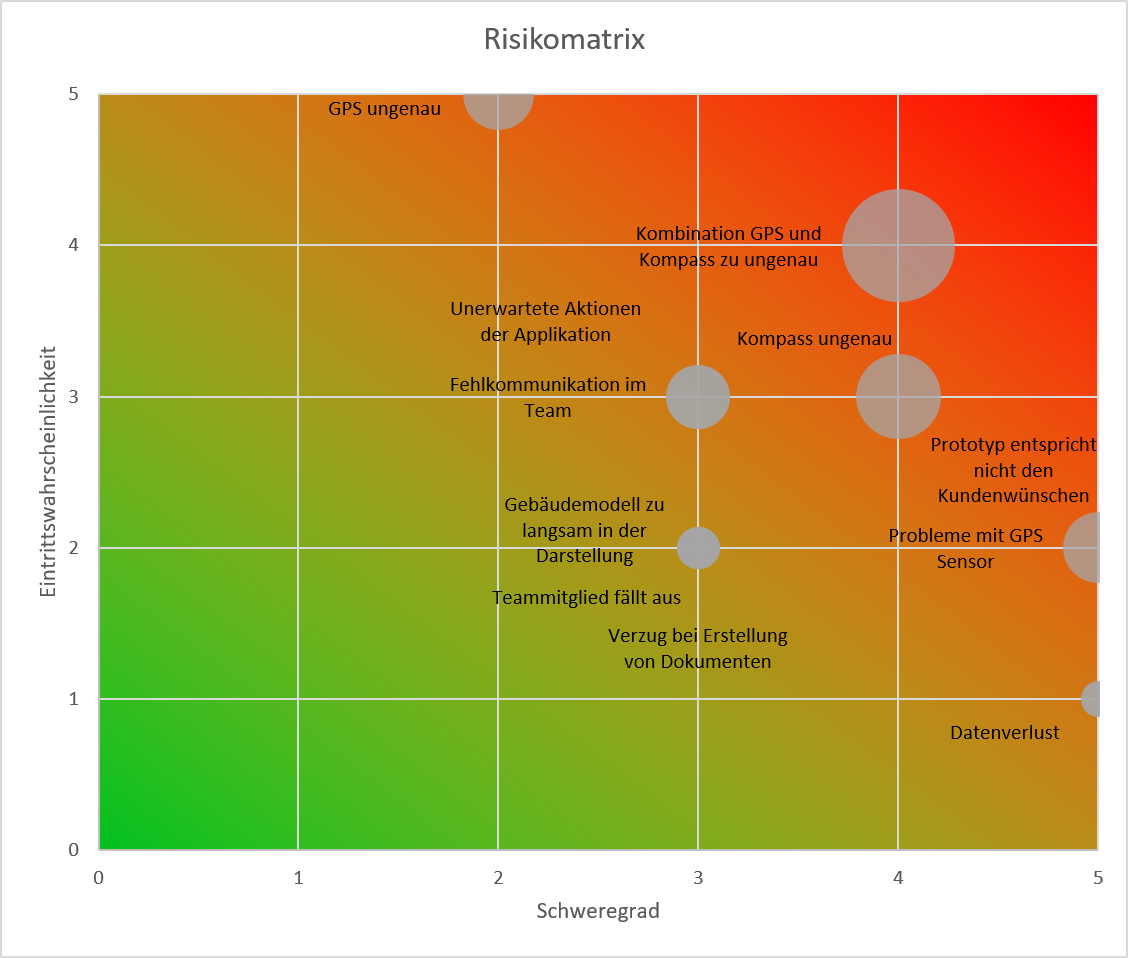
\includegraphics[keepaspectratio, width=0.8\textwidth]{RisikoMatrix}
	\caption{Auswirkungen der Risiken}
\end{figure}

\chapter{Evaluation und Validation}


\chapter{Ausblick}

\appendix

\glossary{Abkürzungsverzeichnis}

\listoffigures

\listoftables

\listofmyequations \pagebreak

\printbibliography

\chapter{Testprotokolle}
\label{appendig:testprotokolle}
\section{Testprotokoll 28.11.2018}
Dieses Protokoll wurde von Dane Wicki am 28.11.2018 erstellt.
\subsection{T-001v1}
Test liefert erwartetes Ergebnis.
\subsection{T-002v1}
Test liefert erwartetes Ergebnis.
\subsection{T-003v2}
Test liefert erwartetes Ergebnis.
\subsection{T-004-v2}
Test liefert erwartetes Ergebnis.
\subsection{T-005-v2}
Test liefert erwartetes Ergebnis.
\subsection{T-006-v2}
Test liefert erwartetes Ergebnis.
\subsection{T-007-v2}
Test liefert erwartetes Ergebnis.
\subsection{T-008-v1}
Test liefert erwartetes Ergebnis.
\subsection{T-009-v2}
Test liefert erwartetes Ergebnis.
\subsection{T-010-v1}
Ausstehend da Bedingungen nicht erfüllt waren.


\chapter{Sprints}

\begin{figure}[h!]
	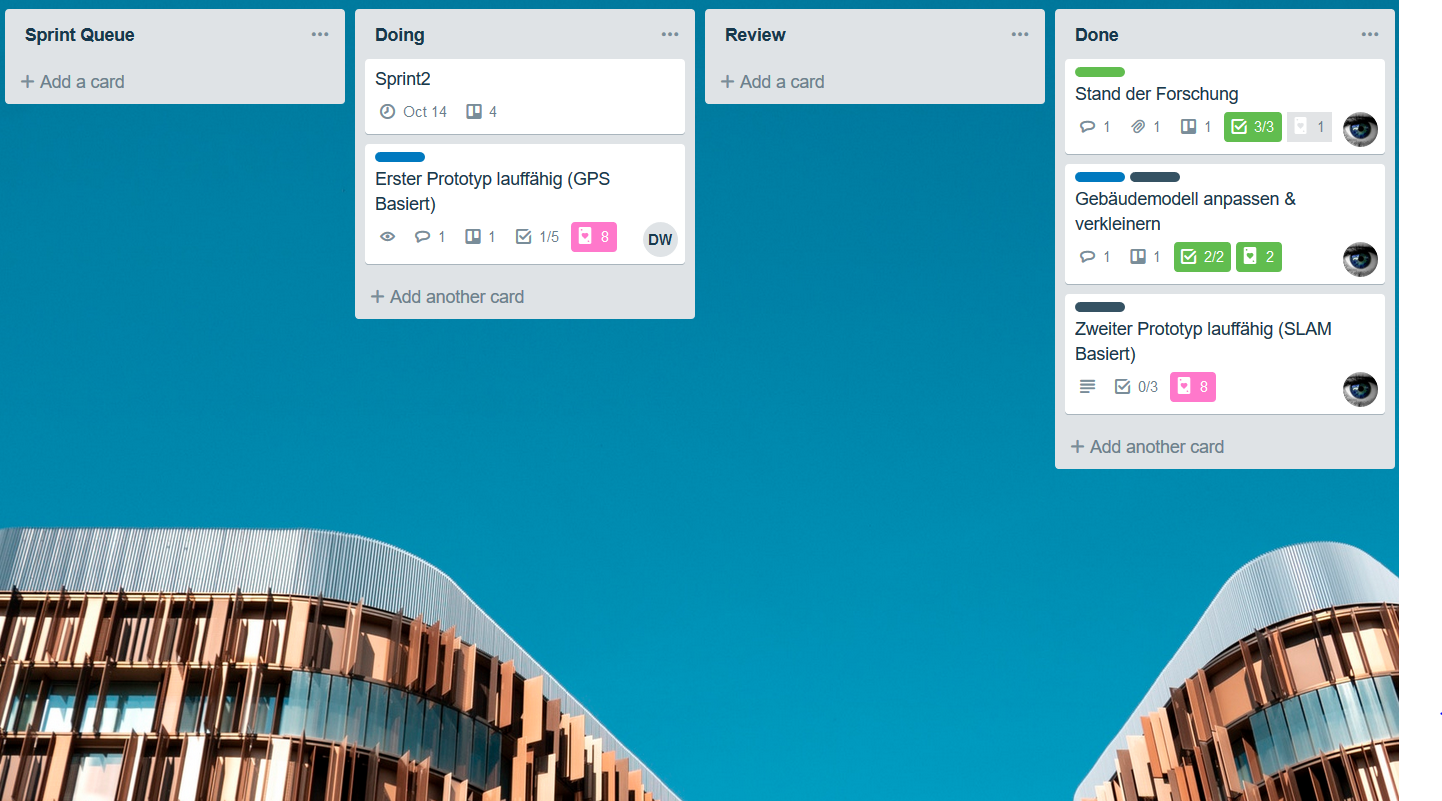
\includegraphics[keepaspectratio,width=\textwidth]{SprintReview_2}
	\caption{Erledigte Tasks in Sprint 2}
\end{figure}

\begin{figure}[h!]
	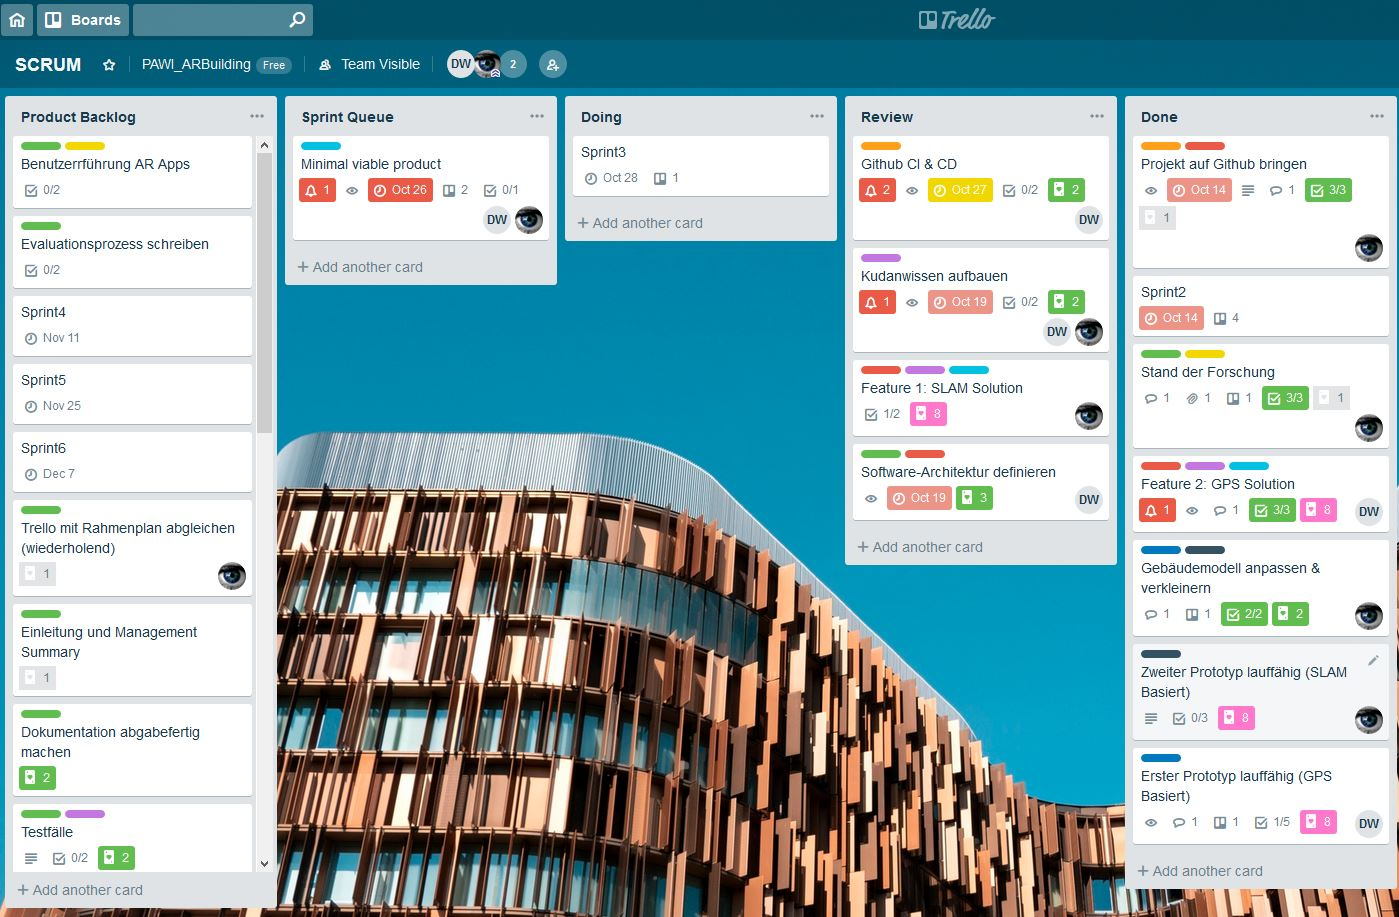
\includegraphics[keepaspectratio,width=\textwidth]{SprintReview_3}
	\caption{Erledigte Tasks in Sprint 3}
\end{figure}

\newpage

\begin{figure}[h!]
	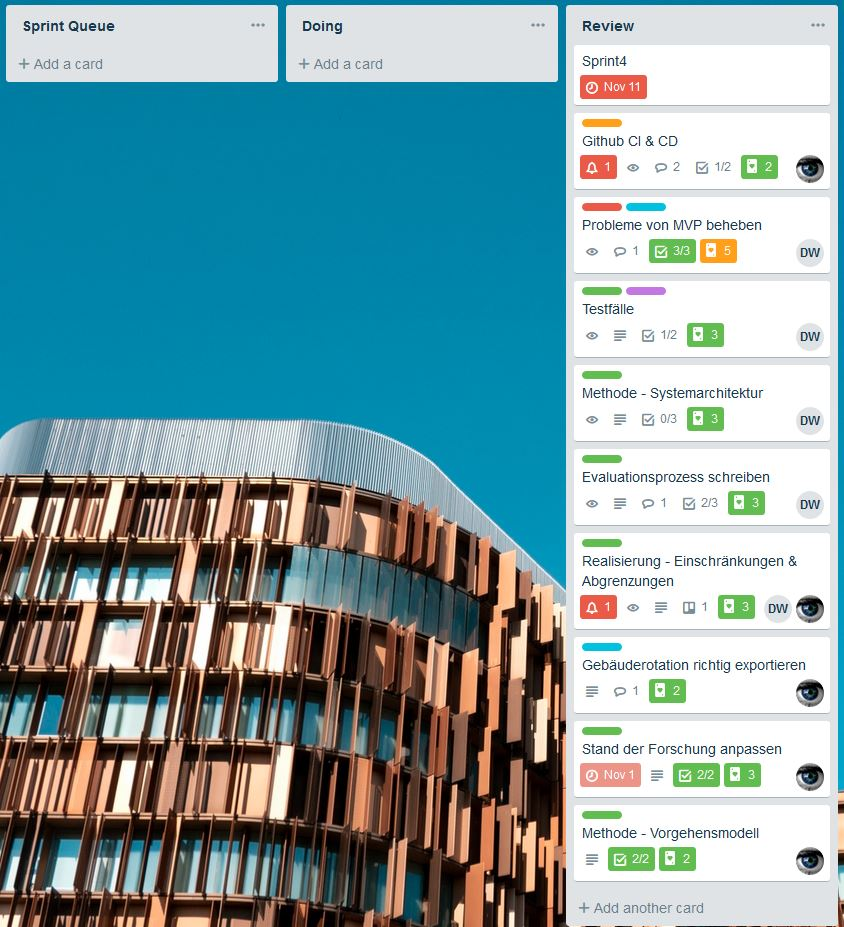
\includegraphics[keepaspectratio,width=\textwidth]{SprintReview_4}
	\caption{Erledigte Tasks in Sprint 4}
\end{figure}

\newpage

\begin{figure}[h!]
	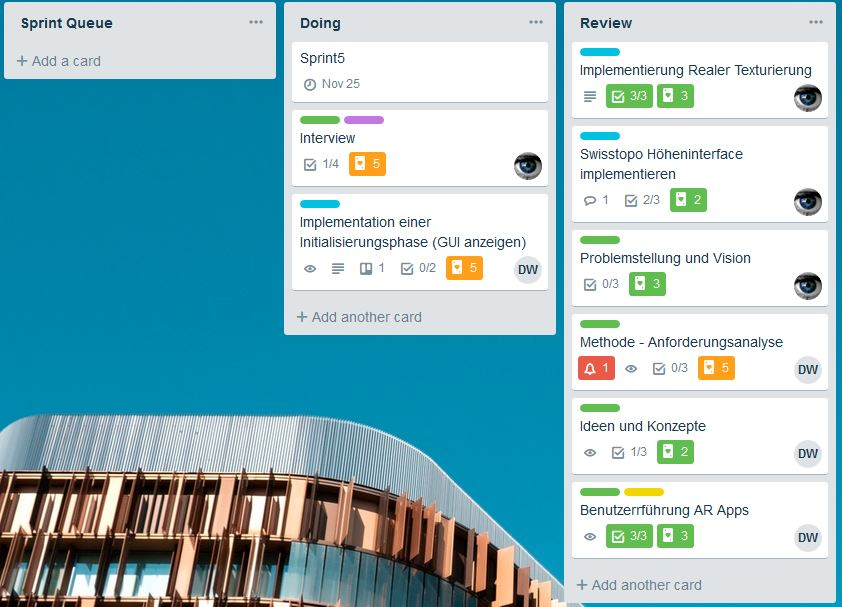
\includegraphics[keepaspectratio,width=\textwidth]{SprintReview_5}
	\caption{Erledigte Tasks in Sprint 5}
\end{figure}

\newpage

\chapter{Evaluationen}

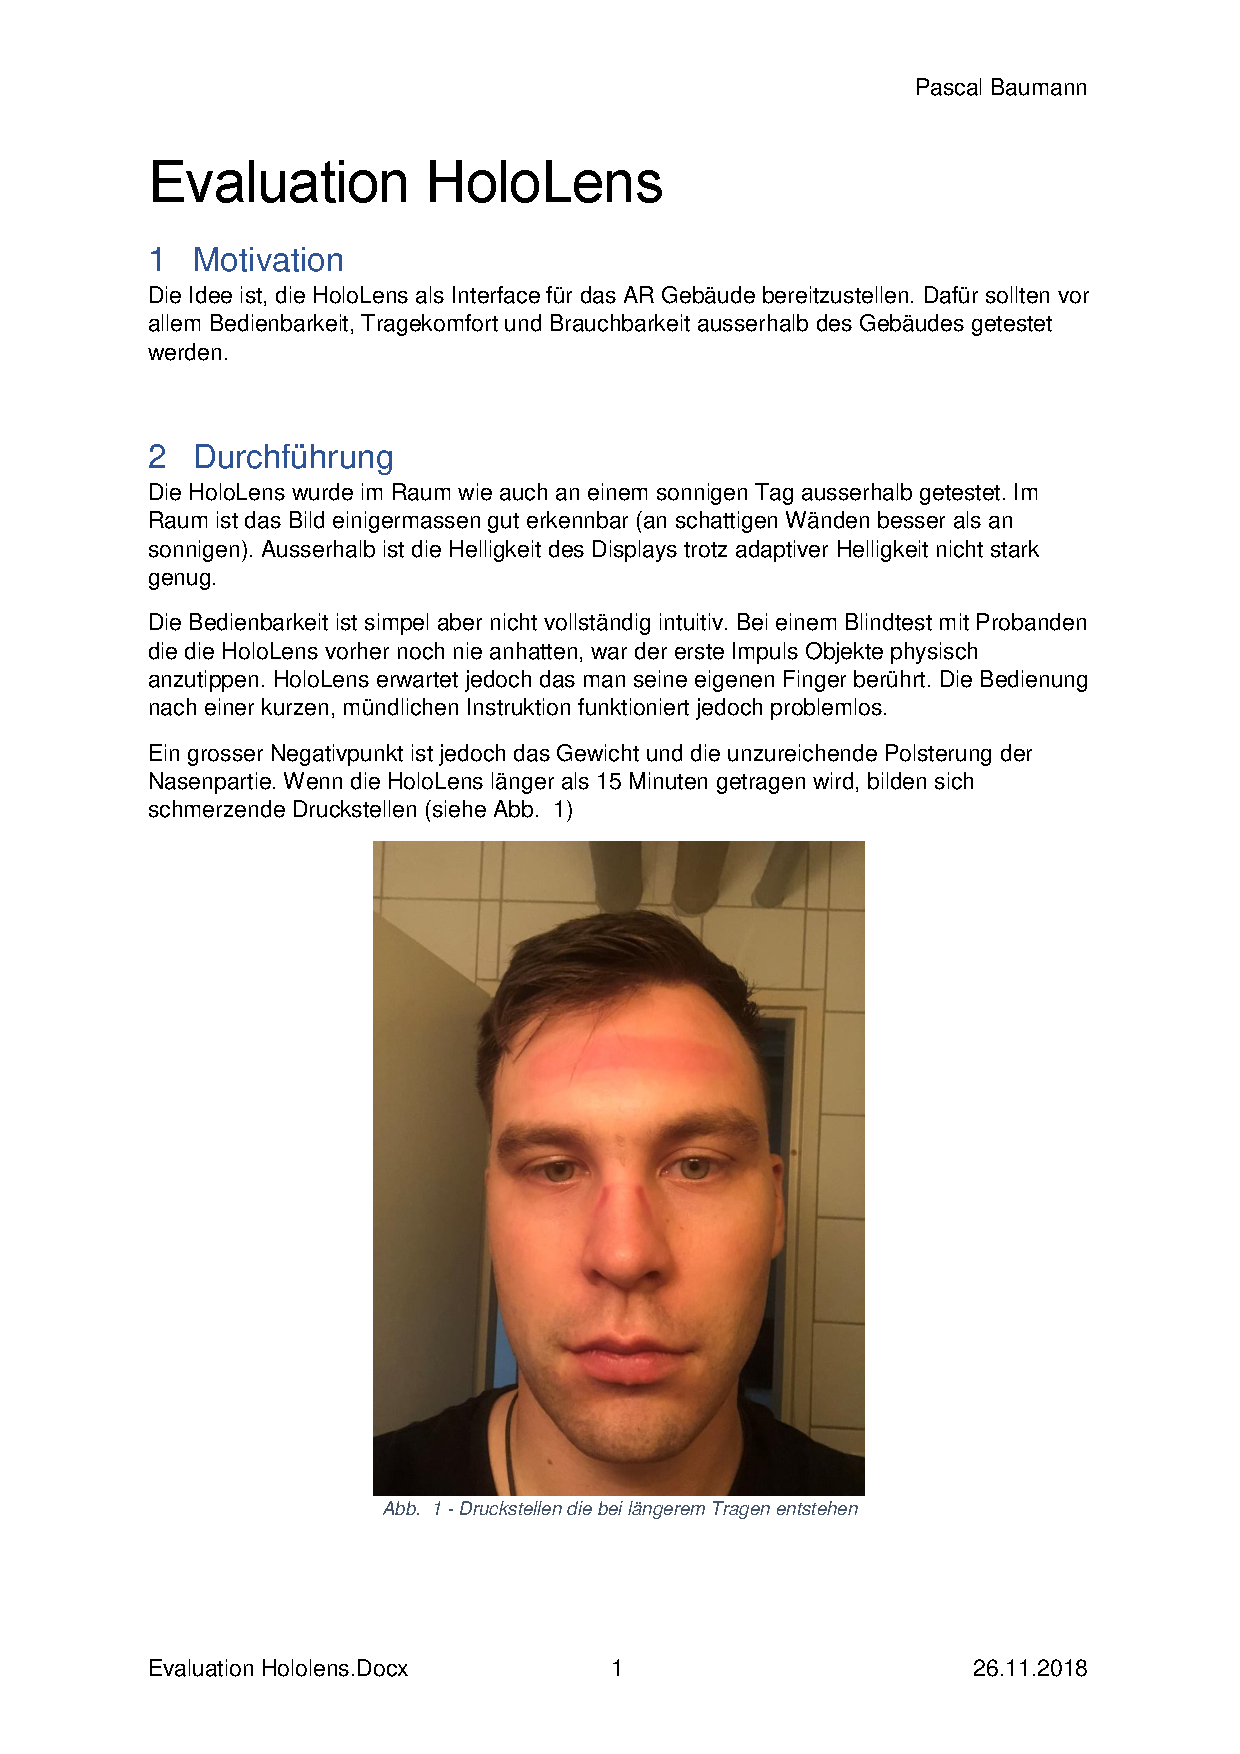
\includepdf[pages=-]{Evaluation_HoloLens.pdf}

\chapter{Anleitungen}

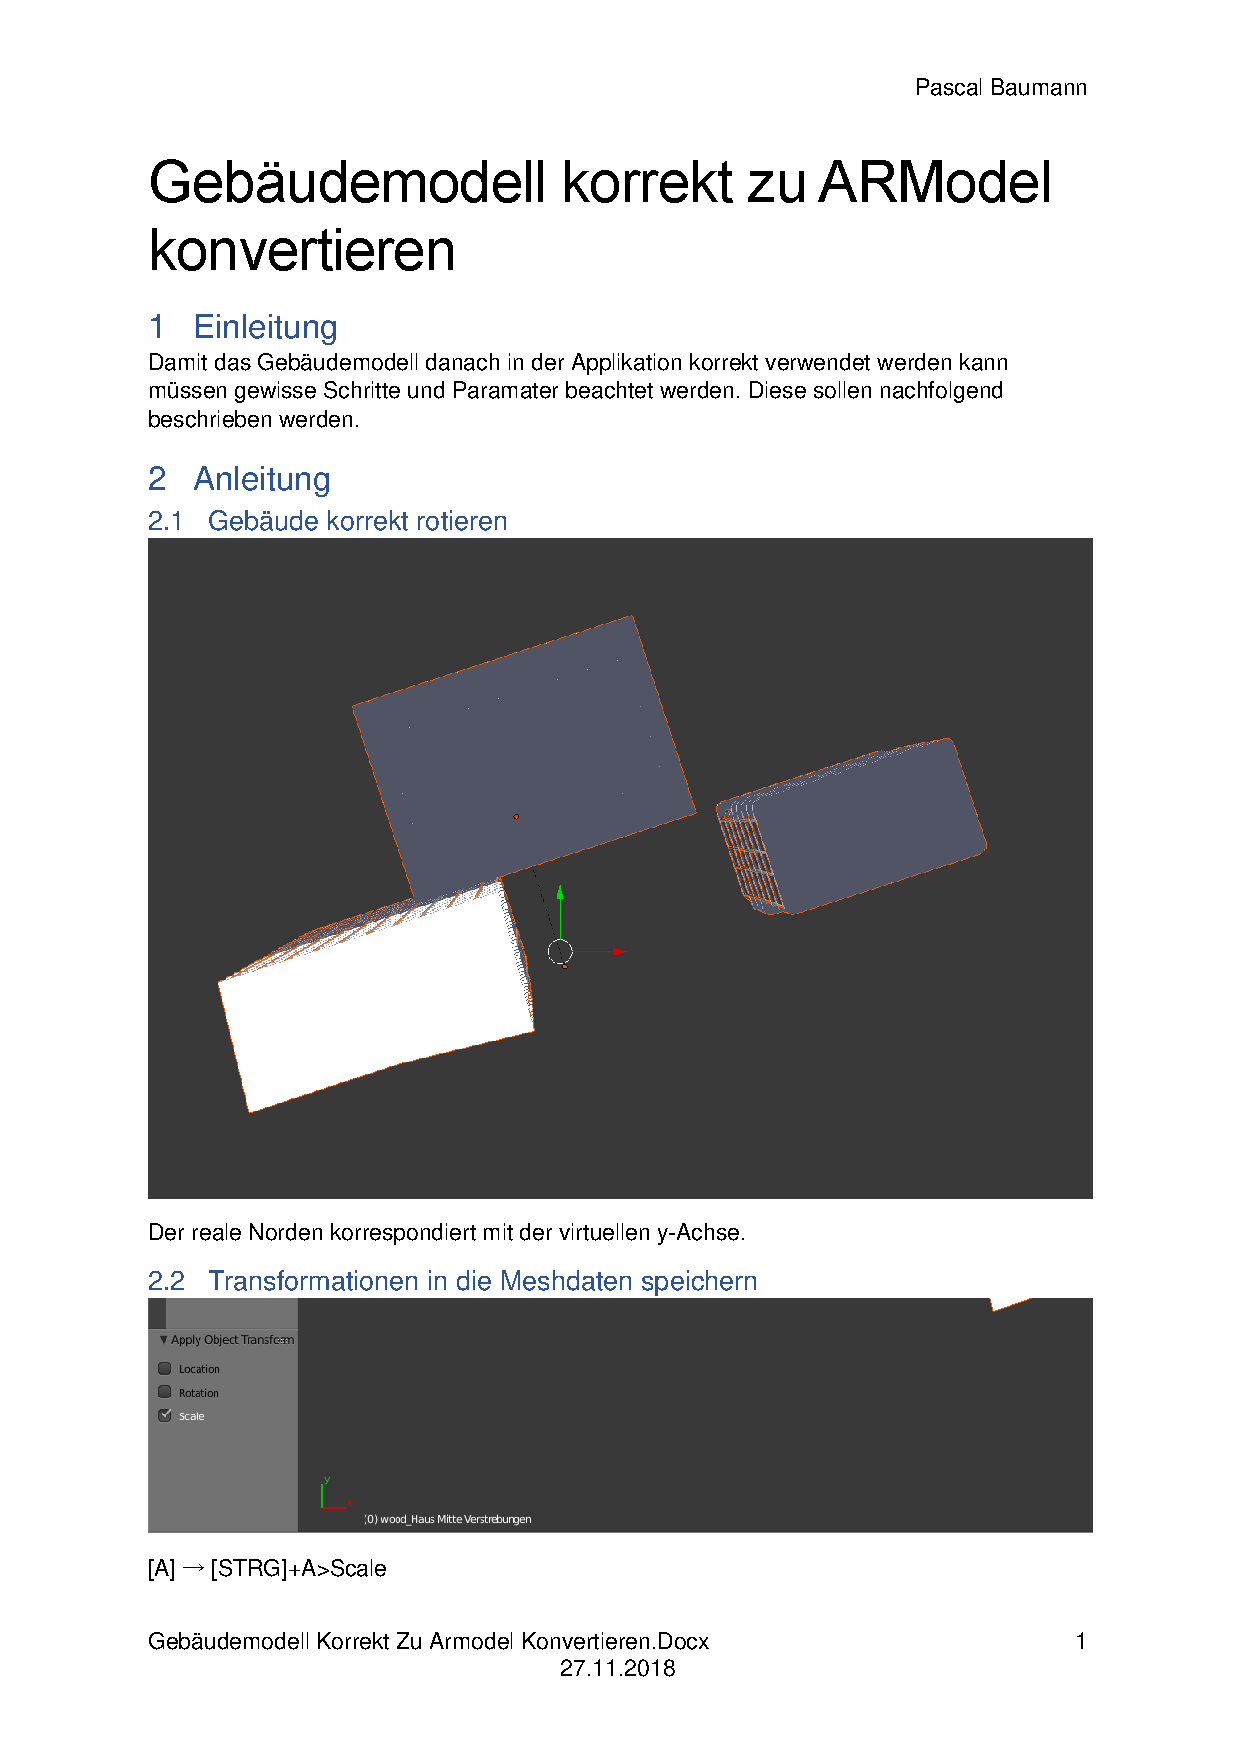
\includepdf[pages=-]{Gebaeudemodell_korrekt_zu_ARModel_konvertieren.pdf}

\chapter*{Eidesstattliche Erklärung}
Ich erkläre hiermit, dass ich/wir die vorliegende Arbeit selbständig und ohne unerlaubte fremde Hilfe angefertigt haben, alle verwendeten Quellen, Literatur und andere Hilfsmittel angegeben haben, wörtlich oder inhaltlich entnommene Stellen als solche kenntlich gemacht haben, das Vertraulichkeitsinteresse des Auftraggebers wahren und die Urheberrechtsbestimmungen der Fachhochschule Zentralschweiz (siehe Merkblatt «Studentische Arbeiten» auf MyCampus) respektieren werden.

\vspace{1em}

\renewcommand{\arraystretch}{2}
\begin{tabularx}{\textwidth}{XXXX}
	Unterschrift: & & Unterschrift: & \\ \cline{2-2}\cline{4-4}
	Baumann, Pascal & & Wicki, Dane & \\
	Datum: & & Ort: & \\
\end{tabularx}

\end{document}
